\chapter{TRIỂN KHAI VÀ KIỂM THỬ HỆ THỐNG NIOS V VỚI DMA}
\label{Chapter3} % Keep label consistent if referenced elsewhere

Chương này trình bày chi tiết quy trình từng bước được thực hiện để triển khai và kiểm thử một Hệ thống trên Chip (\acrshort{soc}) dựa trên bộ xử lý mềm (soft-core processor) Nios V/m của Intel, tích hợp một bộ điều khiển Truy cập Bộ nhớ Trực tiếp (\acrfull{dma}) tùy chỉnh. Nền tảng phần cứng mục tiêu là bo mạch phát triển (development board) Terasic DE10-Standard \cite{terasicDE10Std} trang bị \acrshort{fpga} Intel Cyclone V \acrshort{soc}. Việc triển khai sử dụng Phần mềm Quartus Prime Lite Edition của Intel, Platform Designer (trước đây là Qsys), và \acrshort{ide} Ashling RiscFree™ \cite{ashling_riscfree_guide} cho việc phát triển và gỡ lỗi (debug) phần mềm.

\section{Xây dựng Hệ thống Phần cứng trên Quartus Prime}
\label{sec:build_hardware}

Phần này bao gồm việc tạo dự án Quartus và thiết kế hệ thống phần cứng bằng Platform Designer.

\begin{enumerate}
    \item \textbf{Tạo Dự án Quartus:}
    \begin{itemize}
        \item Khởi động Quartus Prime Lite Edition.
        \item Tạo một dự án mới bằng Trình hướng dẫn Dự án Mới (New Project Wizard) (File -> New Project Wizard...).
        \item Chỉ định thư mục làm việc (working directory) và tên dự án (project name) (ví dụ: \texttt{D:\textbackslash FETEL\_WorkDir\textbackslash Y4S2\_DMANiosVIntern}, \texttt{DMANiosV}) (Hình \ref{fig:03_11}).
        \item Chọn thiết bị mục tiêu (target device) tương ứng với bo mạch DE10-Standard: Họ (Family) `Cyclone V`, Thiết bị (Device) \texttt{5CSXFC6D6F31C6} (Hình \ref{fig:03_12}).
    \end{itemize}
    \item \textbf{Chuẩn bị các tệp Verilog DMA Controller:} Sao chép các tệp nguồn Verilog được cung cấp cho bộ điều khiển DMA (\texttt{DMAController.v} (\ref{app:verilog_dmac}), \texttt{CONTROL\_SLAVE.v} (\ref{app:verilog_control_slave}), \texttt{FIFO\_IP.v}, \texttt{READ\_MASTER.v} (\ref{app:verilog_read_master}), \texttt{WRITE\_MASTER.v} (\ref{app:verilog_write_master})) vào thư mục dự án Quartus (Hình \ref{fig:03_13}).
    \item \textbf{Tạo Hệ thống Platform Designer:}
    \begin{itemize}
        \item Khởi chạy Platform Designer (Tools -> Platform Designer).
        \item \textbf{Thêm Bộ xử lý Nios V/m:} Trong IP Catalog, tìm và thêm "Nios V/m Microcontroller Intel FPGA IP". Trong cấu hình của nó, bật tùy chọn  "Enable Reset from Debug Module" để dễ dàng reset phần mềm khi gỡ lỗi (Hình \ref{fig:03_15}).
        \item \textbf{Thêm Bộ nhớ Trên Chip (On-Chip Memory):} Thêm instances của IP "On-Chip Memory (\acrshort{ram} or \acrshort{rom})". Cấu hình cả hai là \acrshort{ram}. Đặt "Tổng dung lượng bộ nhớ (Total memory size)" cho mỗi bộ nhớ là 131072 byte (128 KB) (Cấu hình ví dụ Hình \ref{fig:03_16}). Một bộ nhớ (\texttt{onchip\_memory2\_0}) cho lệnh (instructions), và bộ nhớ còn lại (\texttt{onchip\_memory2\_1}) sẽ được sử dụng cho dữ liệu (data).
        \item \textbf{Thêm JTAG UART:} Thêm "\acrshort{jtag} \acrshort{uart} Intel FPGA IP" để giao tiếp (communication) giữa bộ xử lý Nios V và máy tính chủ (host PC) thông qua kết nối \acrshort{jtag} (cho việc in ra terminal \texttt{printf}).
        \item \textbf{Tạo IP DMA Controller:}
        \begin{itemize}
            \item Trong IP Catalog, chọn "New Component...".
            \item Trong Component Editor, đặt tên (ví dụ: \texttt{DMA\_Controller}).
            \item Chuyển đến tab "Files". Thêm tất cả các tệp Verilog DMA tùy chỉnh (`.v`). Đặt \texttt{DMAController.v} làm Top-Level File bằng cách nhấp đúp vào "Attributes". 
            \item Nhấp vào "Analyze Synthesis Files" để Quartus tổng hợp các tệp Verilog. Nhấn vào "Copy from Synthesis Files" để điền các tệp mô phỏng (simulation files) (Hình \ref{fig:03_21}).
            \item Chuyển đến tab "Signals". Sau đó cấu hình các tín hiệu như hình \ref{fig:03_23}. 
            \item Chuyển đến tab "Signals \& Interfaces". Đảm bảo các interface được cấu hình như sau (Hình \ref{fig:03_26}, \ref{fig:03_27}):
            \begin{itemize}
                \item Ngõ vào Đồng hồ (Clock input - \texttt{clk}): \texttt{clock\_sink}.
                \item Ngõ vào Reset (\texttt{reset\_n}): \texttt{reset\_sink}.
                \item Associated Clock: \texttt{clk} .
                \item Associated Reset: \texttt{reset\_n}.
            \end{itemize}
            \item Nhấp vào "Finish..." để lưu IP DMA Controller (tệp `.tcl`).
        \end{itemize}
        \item \textbf{Thêm IP DMA Controller vào Hệ thống \acrshort{soc}}.
        \item \textbf{Kết nối các Thành phần:} Thực hiện kết nối như hình \ref{fig:03_28}.
        \item \textbf{Gán Địa chỉ Cơ sở (Assign Base Addresses):} Đi đến menu "System" và chọn "Assign Base Addresses" (Hình \ref{fig:03_29}). Công cụ sẽ tự động gán các địa chỉ không trùng lặp cho tất cả các giao diện slave. Các địa chỉ này được lưu trong thư viện BSP dưới file \textbf{system.h}.
        \item \textbf{Thay Nios V (Vector Reset):} Vector reset (reset vector) của Nios V cần trỏ đến bộ nhớ chứa mã lệnh ban đầu (initial program code memory). 
        \begin{itemize}
            \item Ngắt kết nối \texttt{instruction\_master} khỏi \texttt{onchip\_memory2\_1} (hình \ref{fig:03_30}). 
            \item Mở lại cấu hình Nios V/m (nhấp đúp). Đặt "Bộ nhớ Vector Reset (Reset Agent)" thành \texttt{onchip\_memory2\_0.s1} (hình \ref{fig:03_31}).
        \end{itemize}
        \item \textbf{Lưu Hệ thống:} Lưu hệ thống Platform Designer (\texttt{system.qsys}).
    \end{itemize}
    \item \textbf{Generate HDL:} Trong Platform Designer, nhấp vào nút "Generate HDL..." và nhấp vào "Generate" (Hình \ref{fig:03_34}). Thao tác này tạo ra các tệp Verilog đại diện cho hệ thống \acrshort{soc} được kết nối với nhau. Sau khi tổng hợp thành công, ta tích hợp hệ thống vào thiết kế bằng việc thêm tệp `.qip` vào Project Quartus.
    \item \textbf{Tích hợp Hệ thống vào Project Quartus:}
    \begin{itemize}
        \item Trong Quartus, thêm tệp `.qip` được tạo (\texttt{system/synthesis/system.qip}) vào project (Project -> Add/Remove Files in Project...) (Hình \ref{fig:03_37}, Hình \ref{fig:03_38}).
        \item Tạo một tệp Verilog top-level (\texttt{DMANiosV.v} \ref{lst:verilog_top}) để khởi tạo hệ thống được tạo ra, kết nối các ngõ vào đồng hồ (clock) và reset của hệ thống tương ứng với ngõ vào đồng hồ của \acrshort{fpga} (\texttt{CLOCK\_50}) và một nút reset (\texttt{KEY[0]}) (Hình \ref{fig:03_42}). 
    \end{itemize}
    \item \textbf{Import cấu hình chân (Import Pin Assignments):} Sử dụng tệp gán chân DE10-Standard (`.qsf`) được cung cấp từ FPGAcademy \cite{fpgacademy-qsf}, \cite{fpgacademy-boards}. Trong Quartus, mở menu Assignments -> Import Assignments... (Hình \ref{fig:03_39}). Duyệt đến tệp `.qsf` đã tải xuống và import nó (Hình \ref{fig:03_40}).
    \item \textbf{Biên dịch thiết kế (Compile Design):} Chạy quy trình biên dịch toàn bộ trong Quartus (Processing -> Start Compilation) (Hình \ref{fig:03_41}). Xác minh biên dịch thành công và kiểm tra các gán chân trong Assignment Editor (Assignments -> Assignment Editor) (Hình \ref{fig:03_42}). Thao tác này tạo ra tệp `.sof` cần thiết để lập trình \acrshort{fpga}.
\end{enumerate}

% Figure environments for Section 3.2
\begin{figure}[htbp] \centering 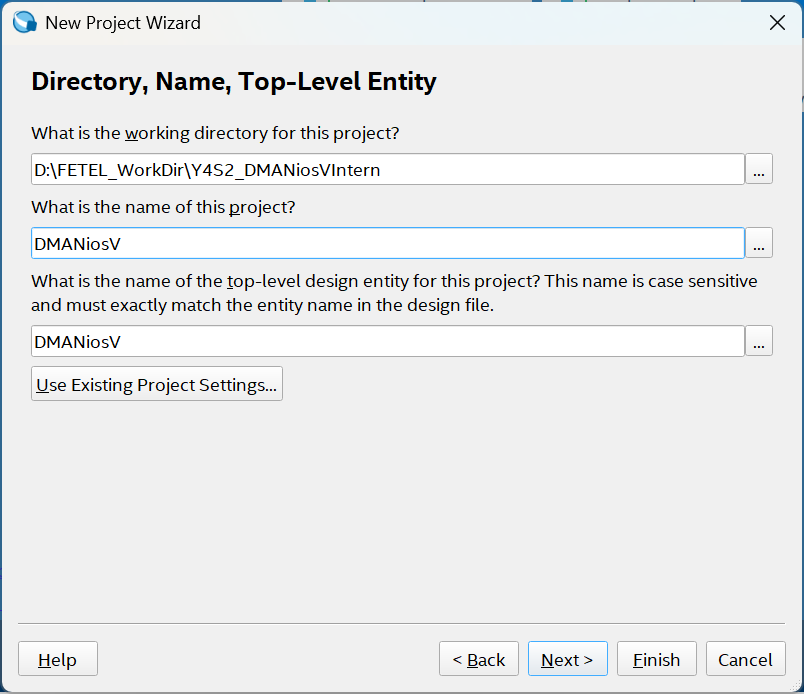
\includegraphics[width=0.7\linewidth]{03_11_QuartusNewProjectWizard1.png} \caption{Quartus: New Project Wizard: Chỉ định đường dẫn thư mục và tên Project.} \label{fig:03_11} \end{figure}
\begin{figure}[htbp] \centering 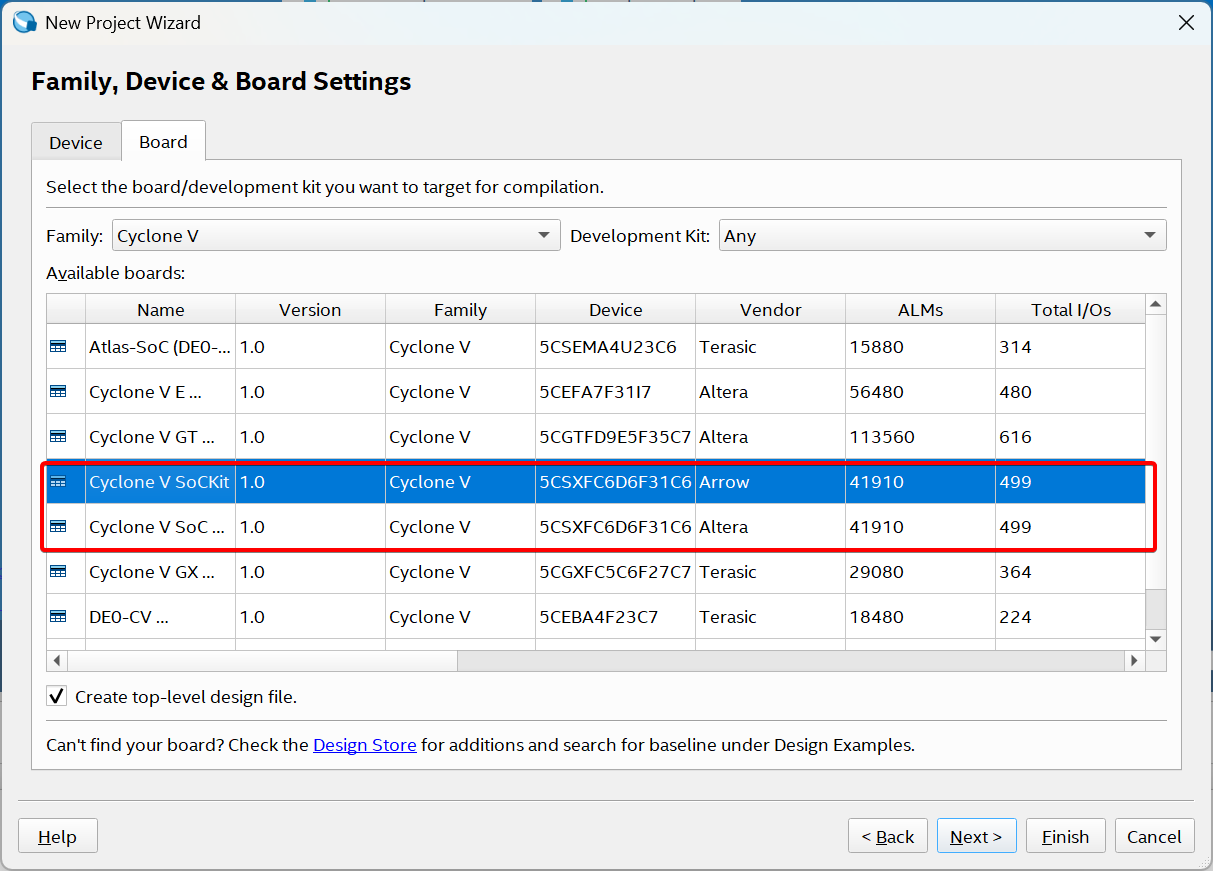
\includegraphics[width=0.9\linewidth]{03_12_QuartusNewProjectWizard2.png} \caption{Quartus: New Project Wizard: Device Selector} \label{fig:03_12} \end{figure}
\begin{figure}[htbp] \centering 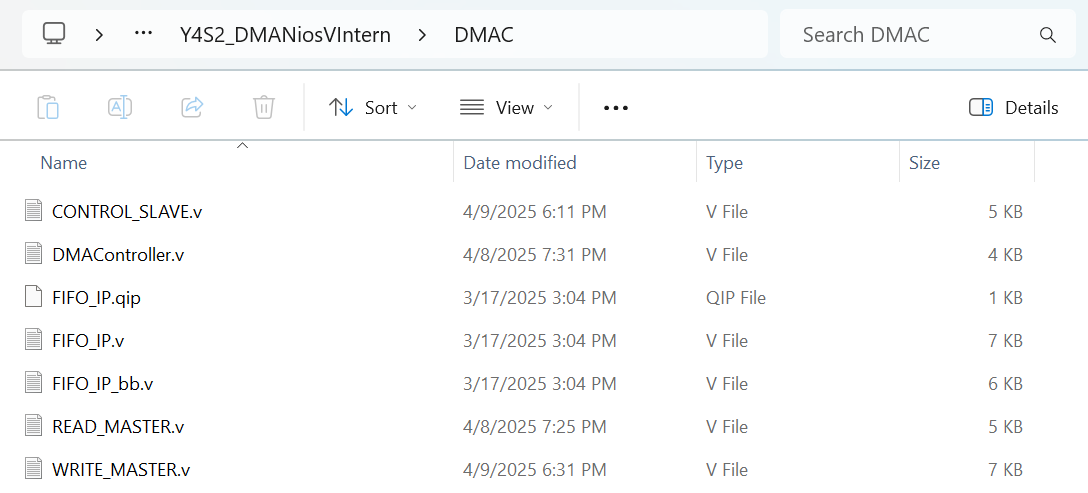
\includegraphics[width=0.9\linewidth]{03_13_ProjectFilesDMA.png} \caption{Thư mục dự án hiển thị các tệp Verilog DMA tùy chỉnh đã sao chép.} \label{fig:03_13} \end{figure}
% \begin{figure}[htbp] \centering 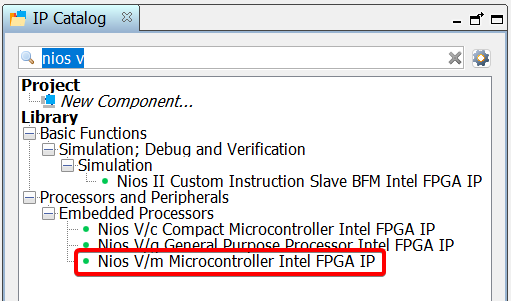
\includegraphics[width=0.6\linewidth]{03_14_IPCatalogNiosVSelection.png} \caption{Platform Designer IP Catalog: Chọn Nios V/m Microcontroller.} \label{fig:03_14} \end{figure}
\begin{figure}[htbp] \centering 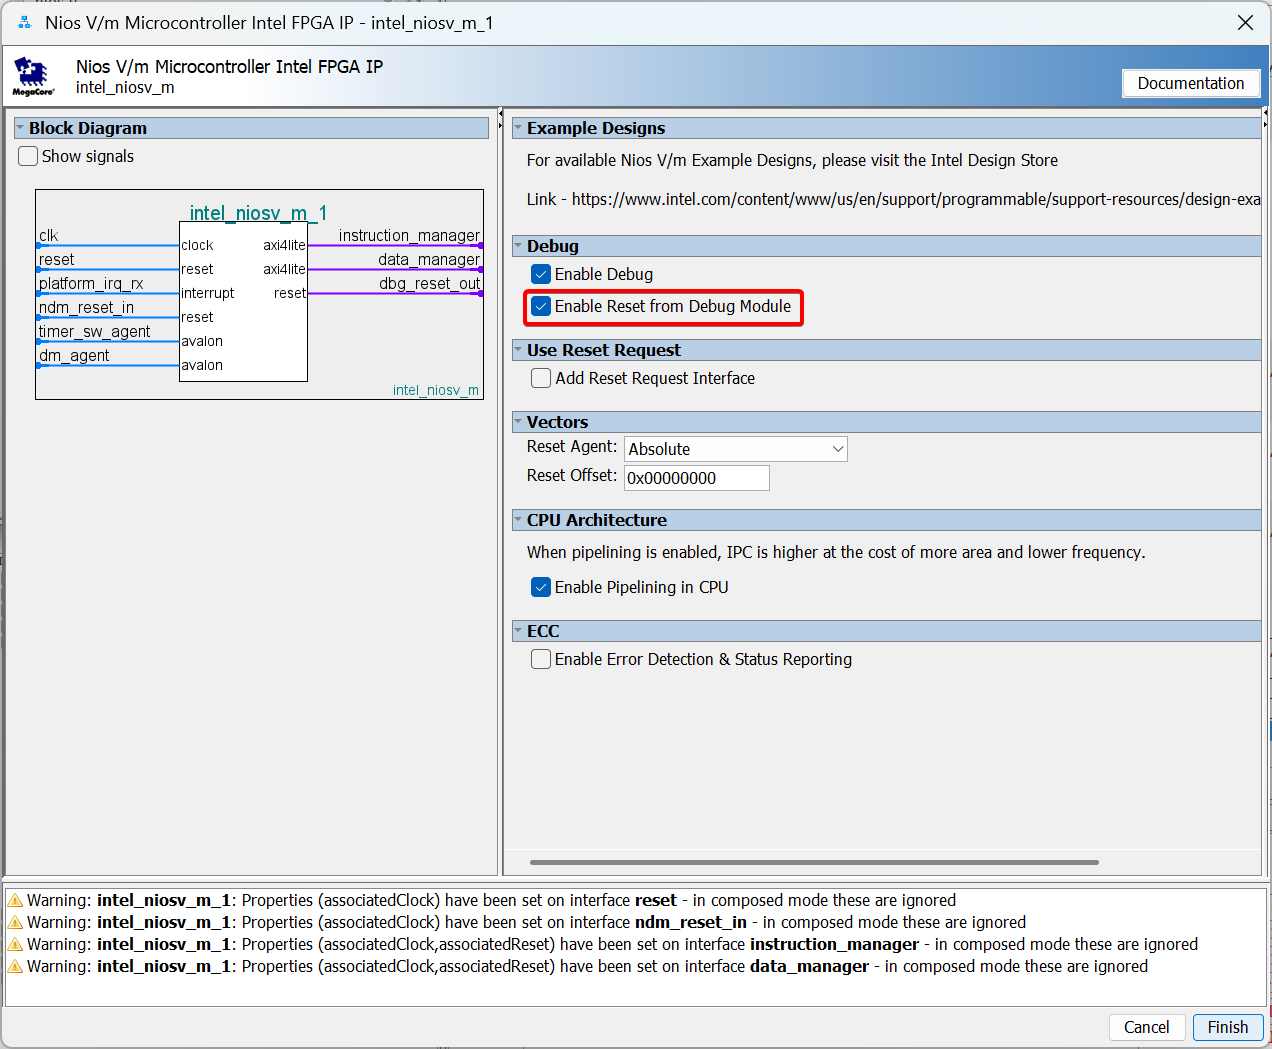
\includegraphics[width=0.9\linewidth]{03_15_NiosVIPConfig1.png} \caption{Cấu hình IP Nios V/m: Bật "Enable Reset from Debug Module".} \label{fig:03_15} \end{figure}
\begin{figure}[htbp] \centering 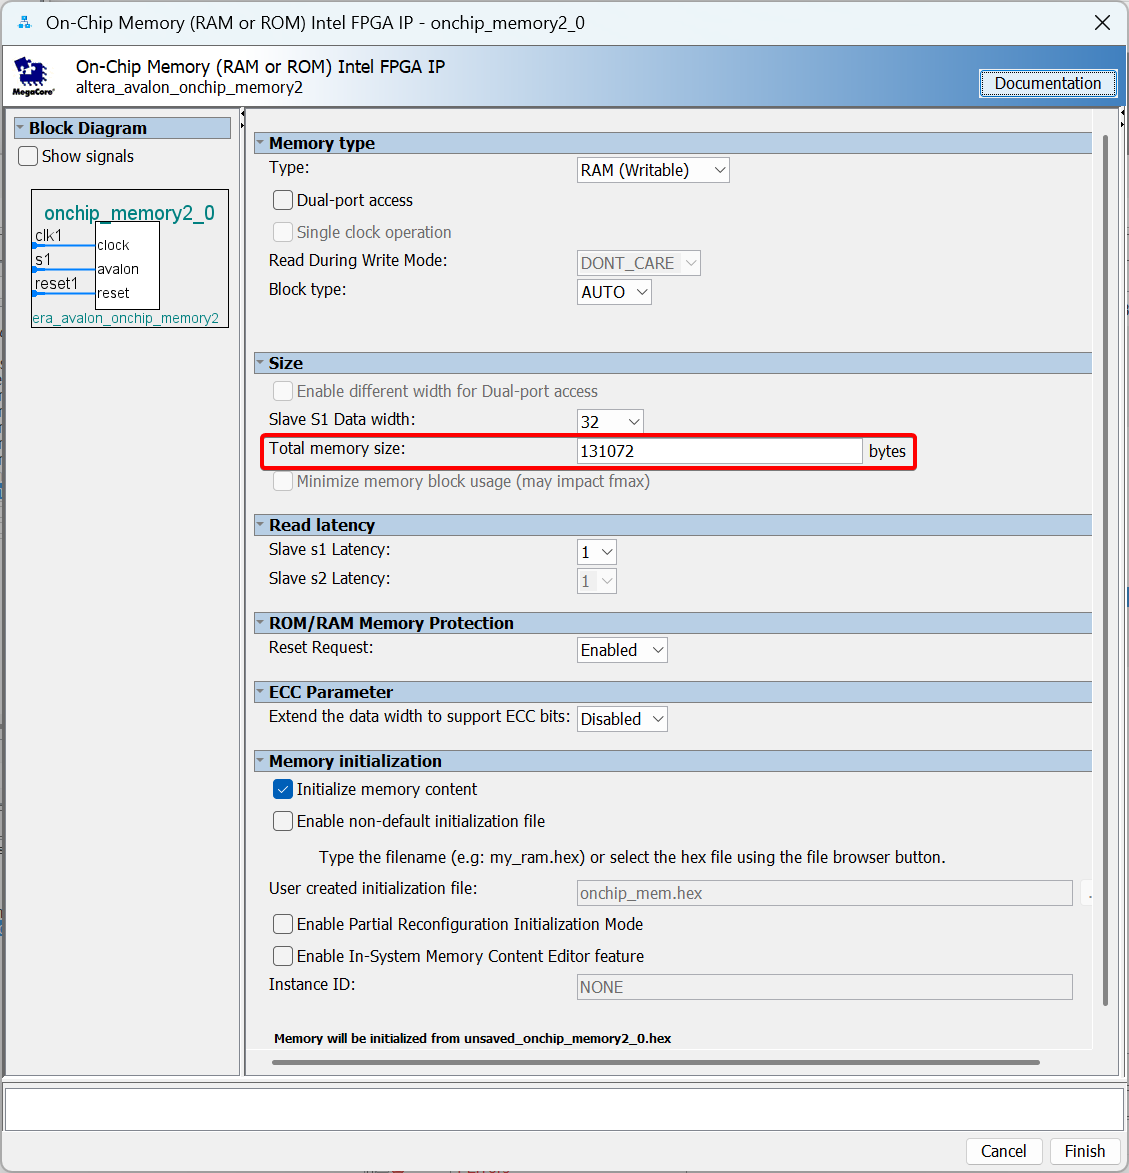
\includegraphics[width=0.9\linewidth]{03_16_OnChipMemoryIPConfig.png} \caption{Cấu hình IP Bộ nhớ Trên Chip: Đặt kích thước thành 128 KB.} \label{fig:03_16} \end{figure}
\begin{figure}[htbp] \centering 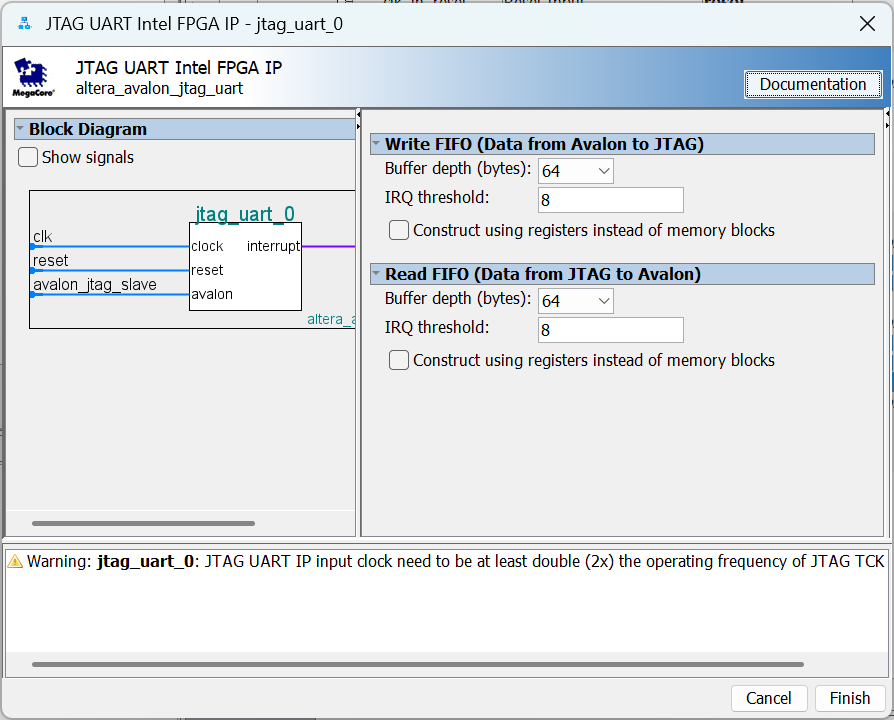
\includegraphics[width=0.9\linewidth]{03_17_JTAGUARTIPConfig.png} \caption{Cấu hình IP JTAG UART.} \label{fig:03_17} \end{figure}
% \begin{figure}[htbp] \centering 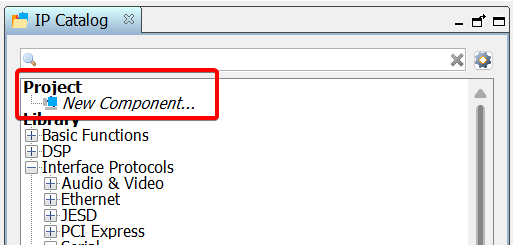
\includegraphics[width=0.6\linewidth]{03_18_IPCatalog_AddComponent.png} \caption{IP Catalog Platform Designer: Chọn "New Component...".} \label{fig:03_18} \end{figure}
% \begin{figure}[htbp] \centering 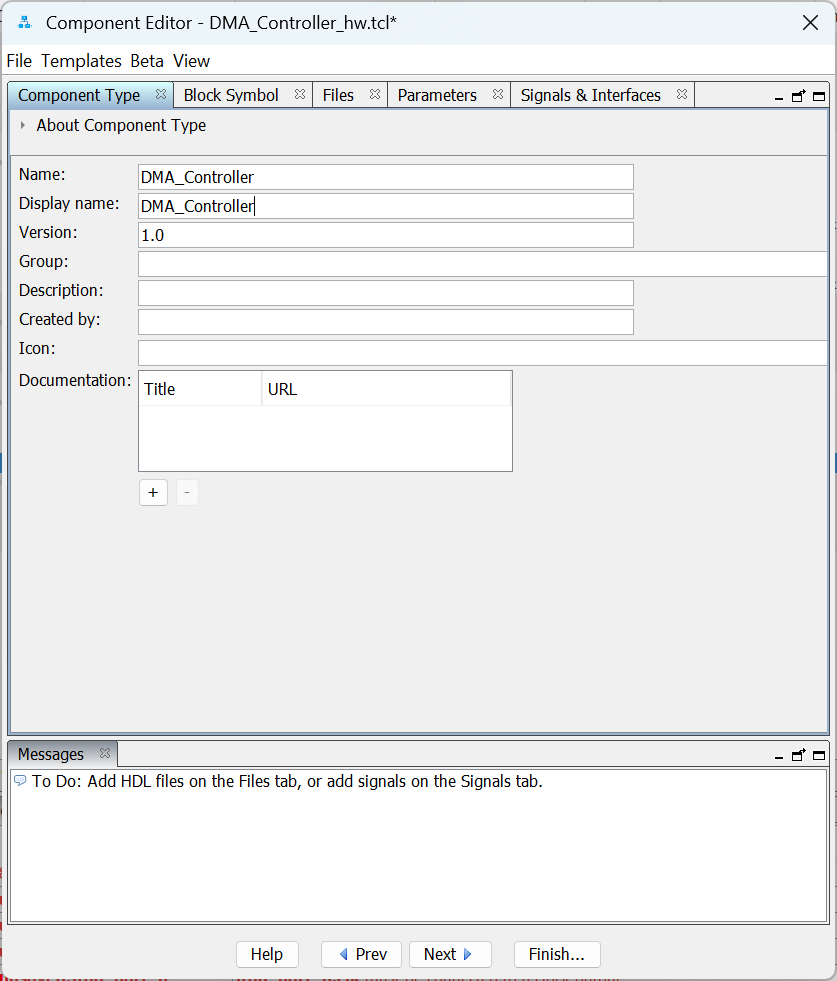
\includegraphics[width=0.9\linewidth]{03_19_ComponentEditorType.png} \caption{Component Editor: Đặt tên cho thành phần DMA tùy chỉnh.} \label{fig:03_19} \end{figure}
% \begin{figure}[htbp] \centering 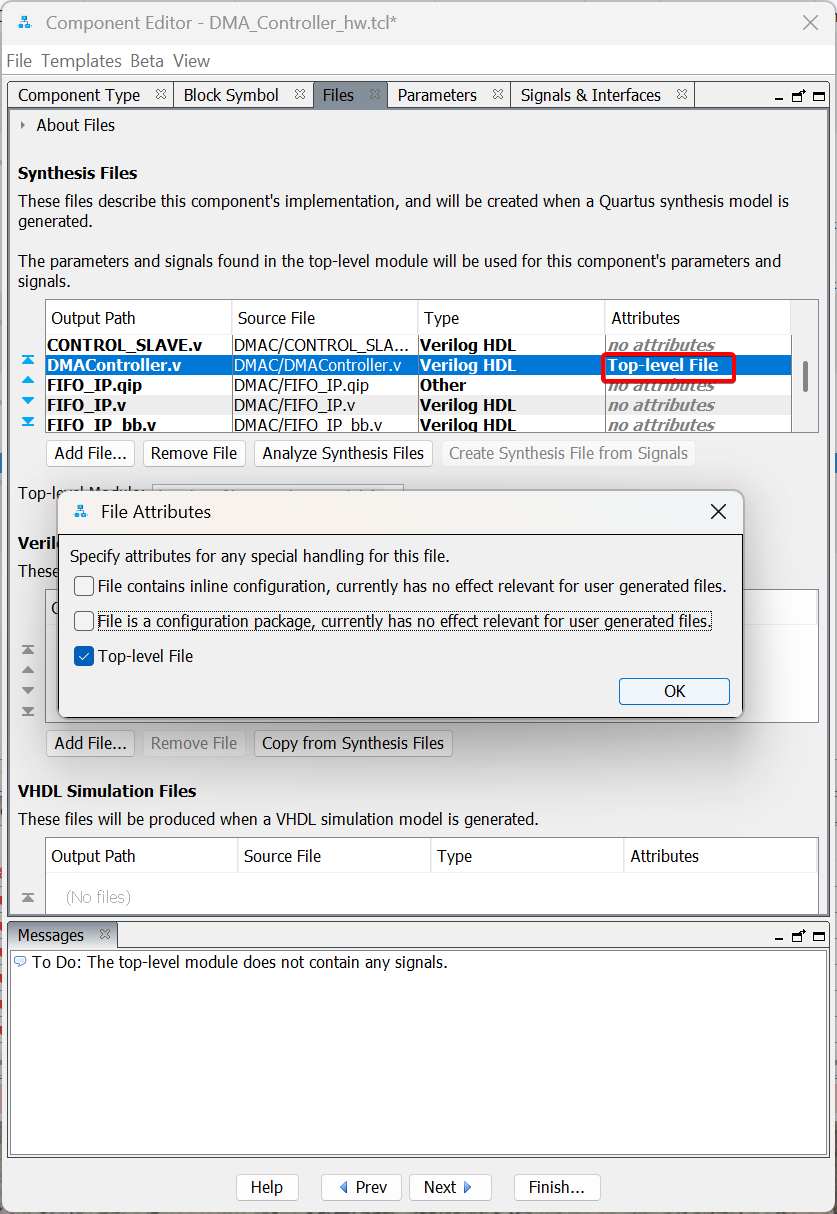
\includegraphics[width=0.9\linewidth]{03_20_ComponentEditorFiles_TopLevel.png} \caption{Component Editor: Thêm tệp Verilog và đặt top-level.} \label{fig:03_20} \end{figure}
\begin{figure}[htbp] \centering 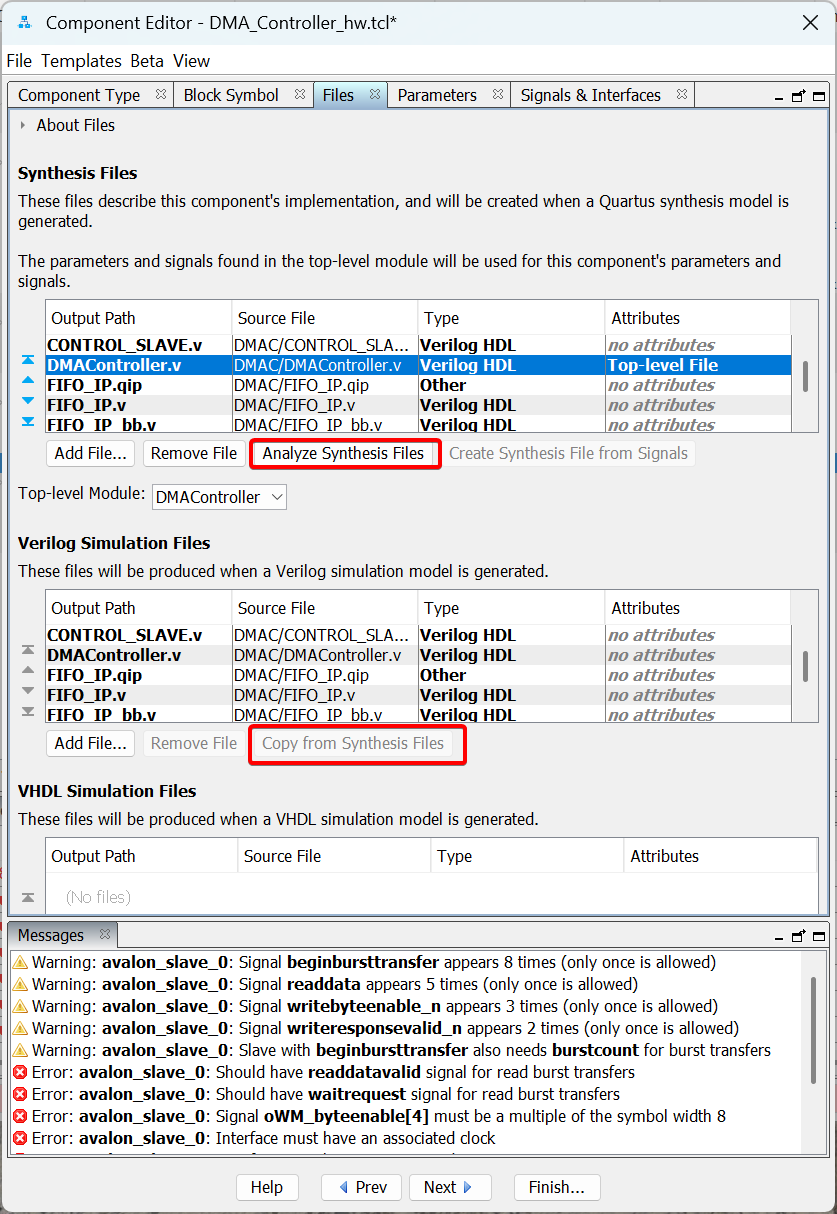
\includegraphics[width=0.9\linewidth]{03_21_ComponentEditorFilesAnalyzed.png} \caption{Component Editor: Các tệp sau khi Phân tích và Sao chép từ Tổng hợp.} \label{fig:03_21} \end{figure}
% \begin{figure}[htbp] \centering 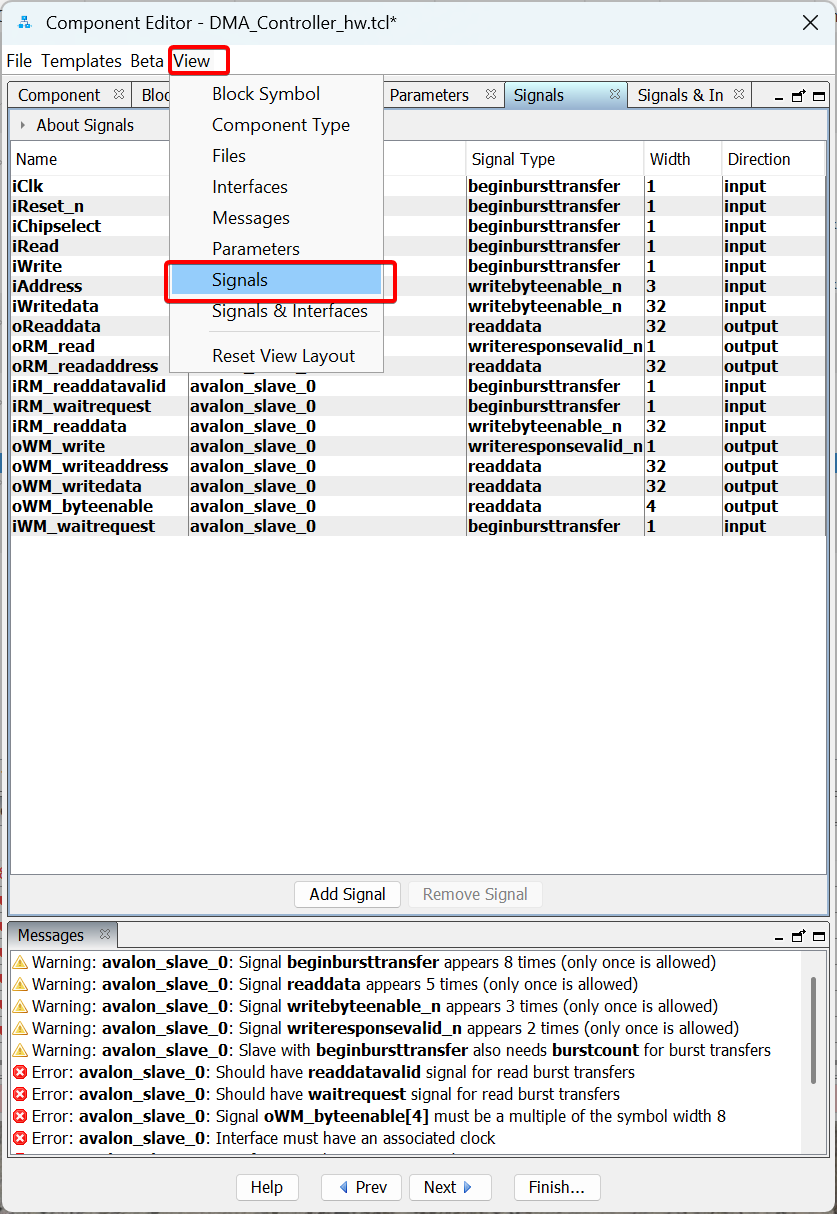
\includegraphics[width=0.9\linewidth]{03_22_ComponentEditorSignals1.png} \caption{Component Editor: Tab Tín hiệu \& Giao diện ban đầu hiển thị cảnh báo.} \label{fig:03_22} \end{figure}
\begin{figure}[htbp] \centering 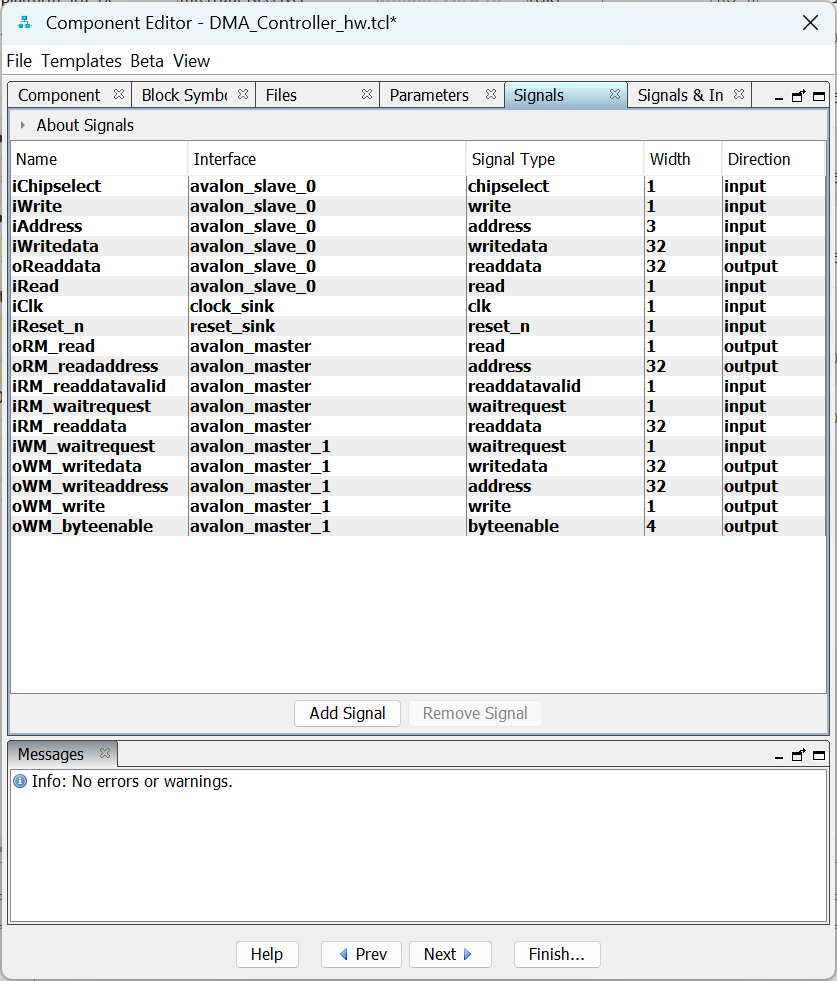
\includegraphics[width=0.9\linewidth]{03_23_ComponentEditorSignals_DMAC.png} \caption{Component Editor: Các loại tín hiệu clock và reset đã được sửa.} \label{fig:03_23} \end{figure}
% \begin{figure}[htbp] \centering 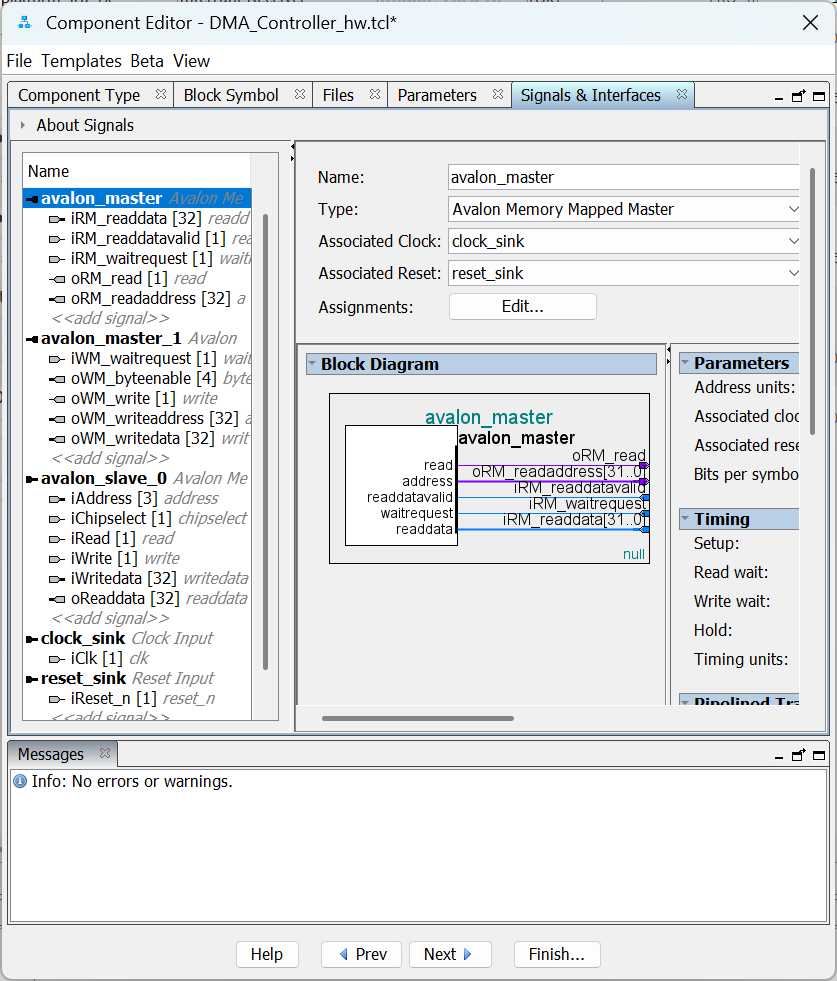
\includegraphics[width=0.5\linewidth]{03_24_ComponentEditorInterfaces1.png} \caption{Component Editor: Định nghĩa giao diện Avalon Master.} \label{fig:03_24} \end{figure}
% \begin{figure}[htbp] \centering 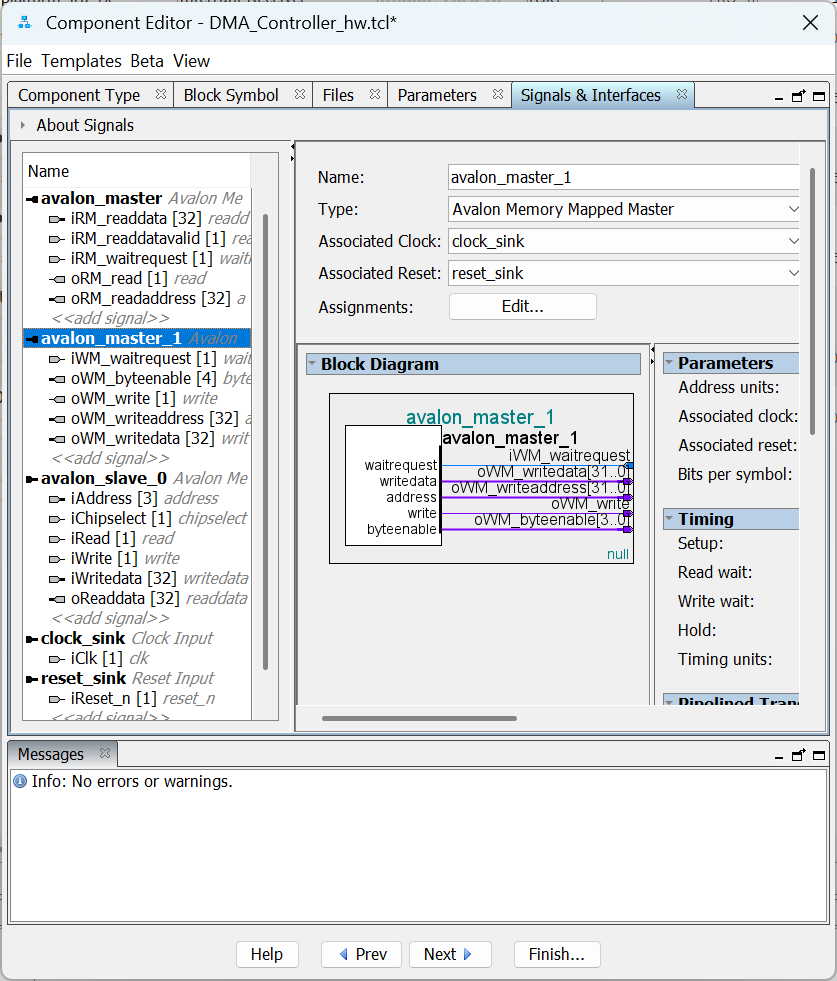
\includegraphics[width=0.5\linewidth]{03_25_ComponentEditorInterfaces2.png} \caption{Component Editor: Chế độ xem sơ đồ khối giao diện Avalon Master.} \label{fig:03_25} \end{figure}
\begin{figure}[htbp] \centering 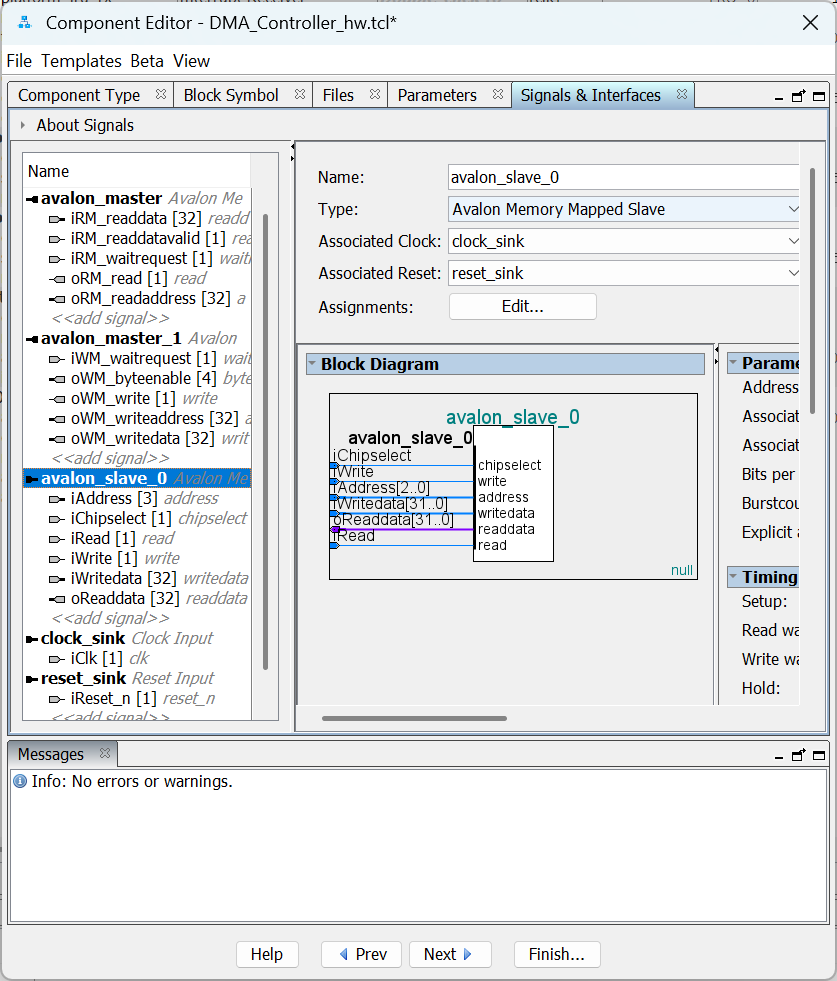
\includegraphics[width=0.5\linewidth]{03_26_ComponentEditorInterfaces3.png} \caption{Component Editor: Chế độ xem sơ đồ khối giao diện Avalon Slave.} \label{fig:03_26} \end{figure}
\begin{figure}[htbp] \centering 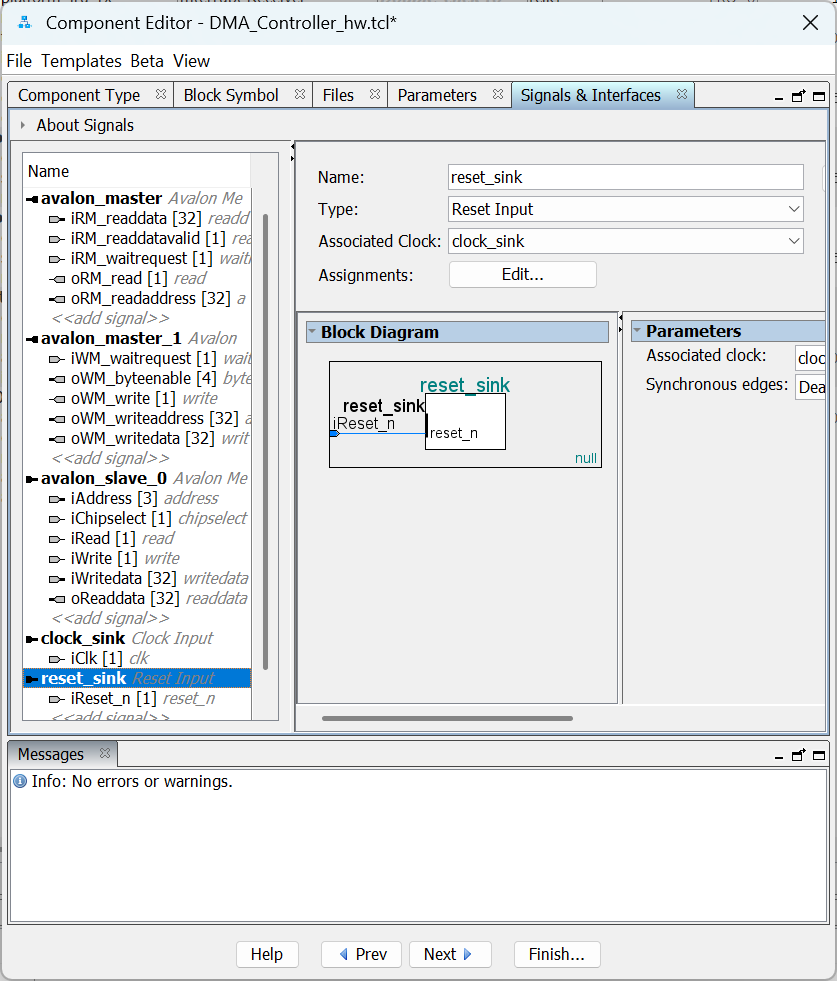
\includegraphics[width=0.5\linewidth]{03_27_ComponentEditorInterfaces4.png} \caption{Component Editor: Chế độ xem giao diện Reset và Clock sink.} \label{fig:03_27} \end{figure}
\begin{figure}[htbp] \centering 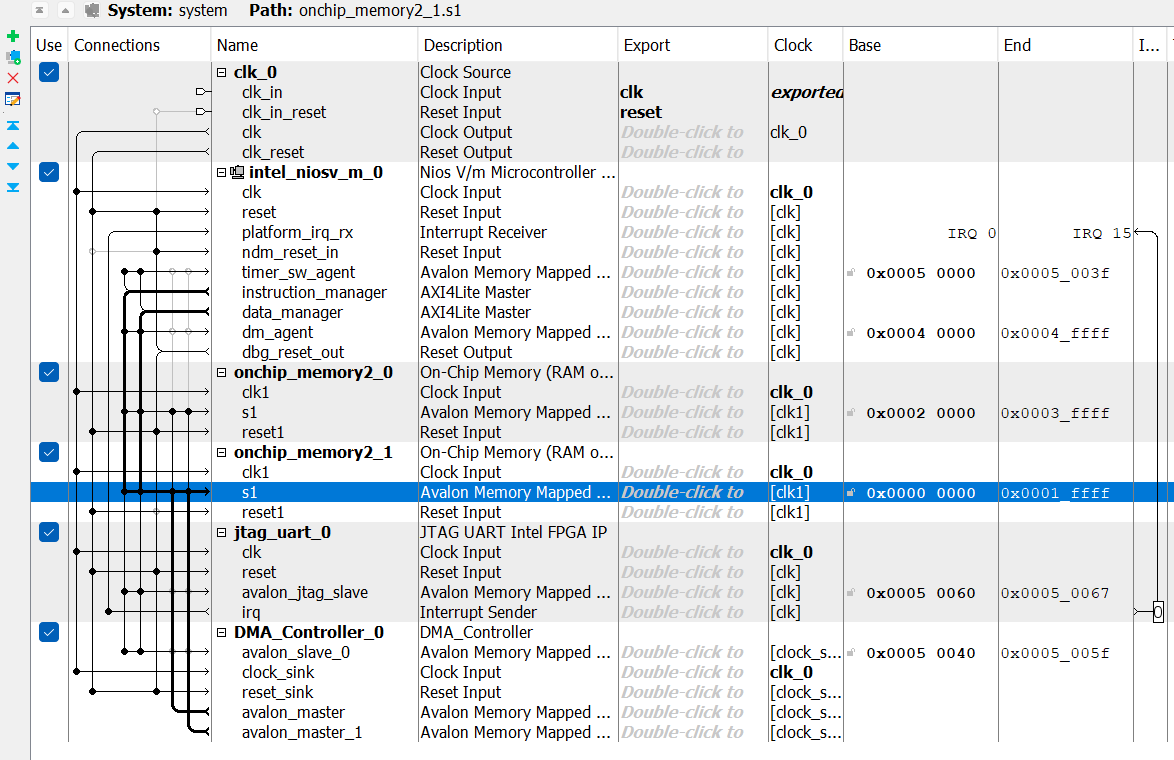
\includegraphics[width=\linewidth]{03_28_PlatformDesignerSystemView1.png} \caption{Platform Designer: Hệ thống có kết nối giữa \texttt{instruction\_master} với s1 (của \texttt{onchip\_memory2\_1}).} \label{fig:03_28} \end{figure}
\begin{figure}[htbp] \centering 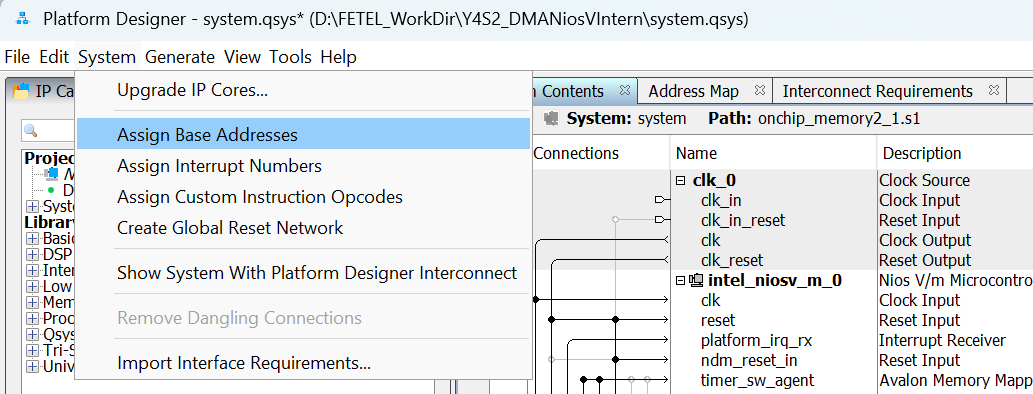
\includegraphics[width=\linewidth]{03_29_PlatformDesignerAssignBaseAddr.png} \caption{Platform Designer: Gán Địa chỉ Cơ sở (Assign Base Addresses).} \label{fig:03_29} \end{figure}
\begin{figure}[htbp] \centering 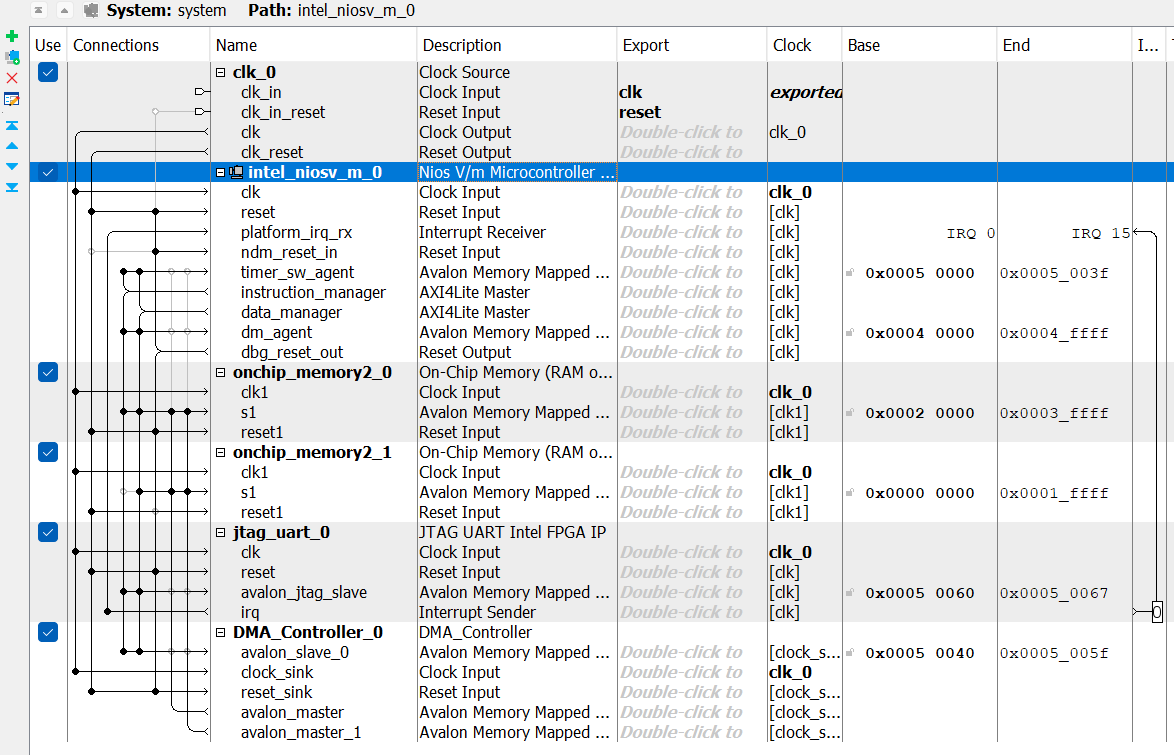
\includegraphics[width=\linewidth]{03_30_PlatformDesignerSystemView_FinalDMAC.png} \caption{Platform Designer: Mô hình hệ thống hoàn chỉnh (sau khi ngắt kết nối \texttt{instruction\_master} với \texttt{s1} trên \texttt{onchip\_memory2\_1}).} \label{fig:03_30} \end{figure}
\begin{figure}[htbp] \centering 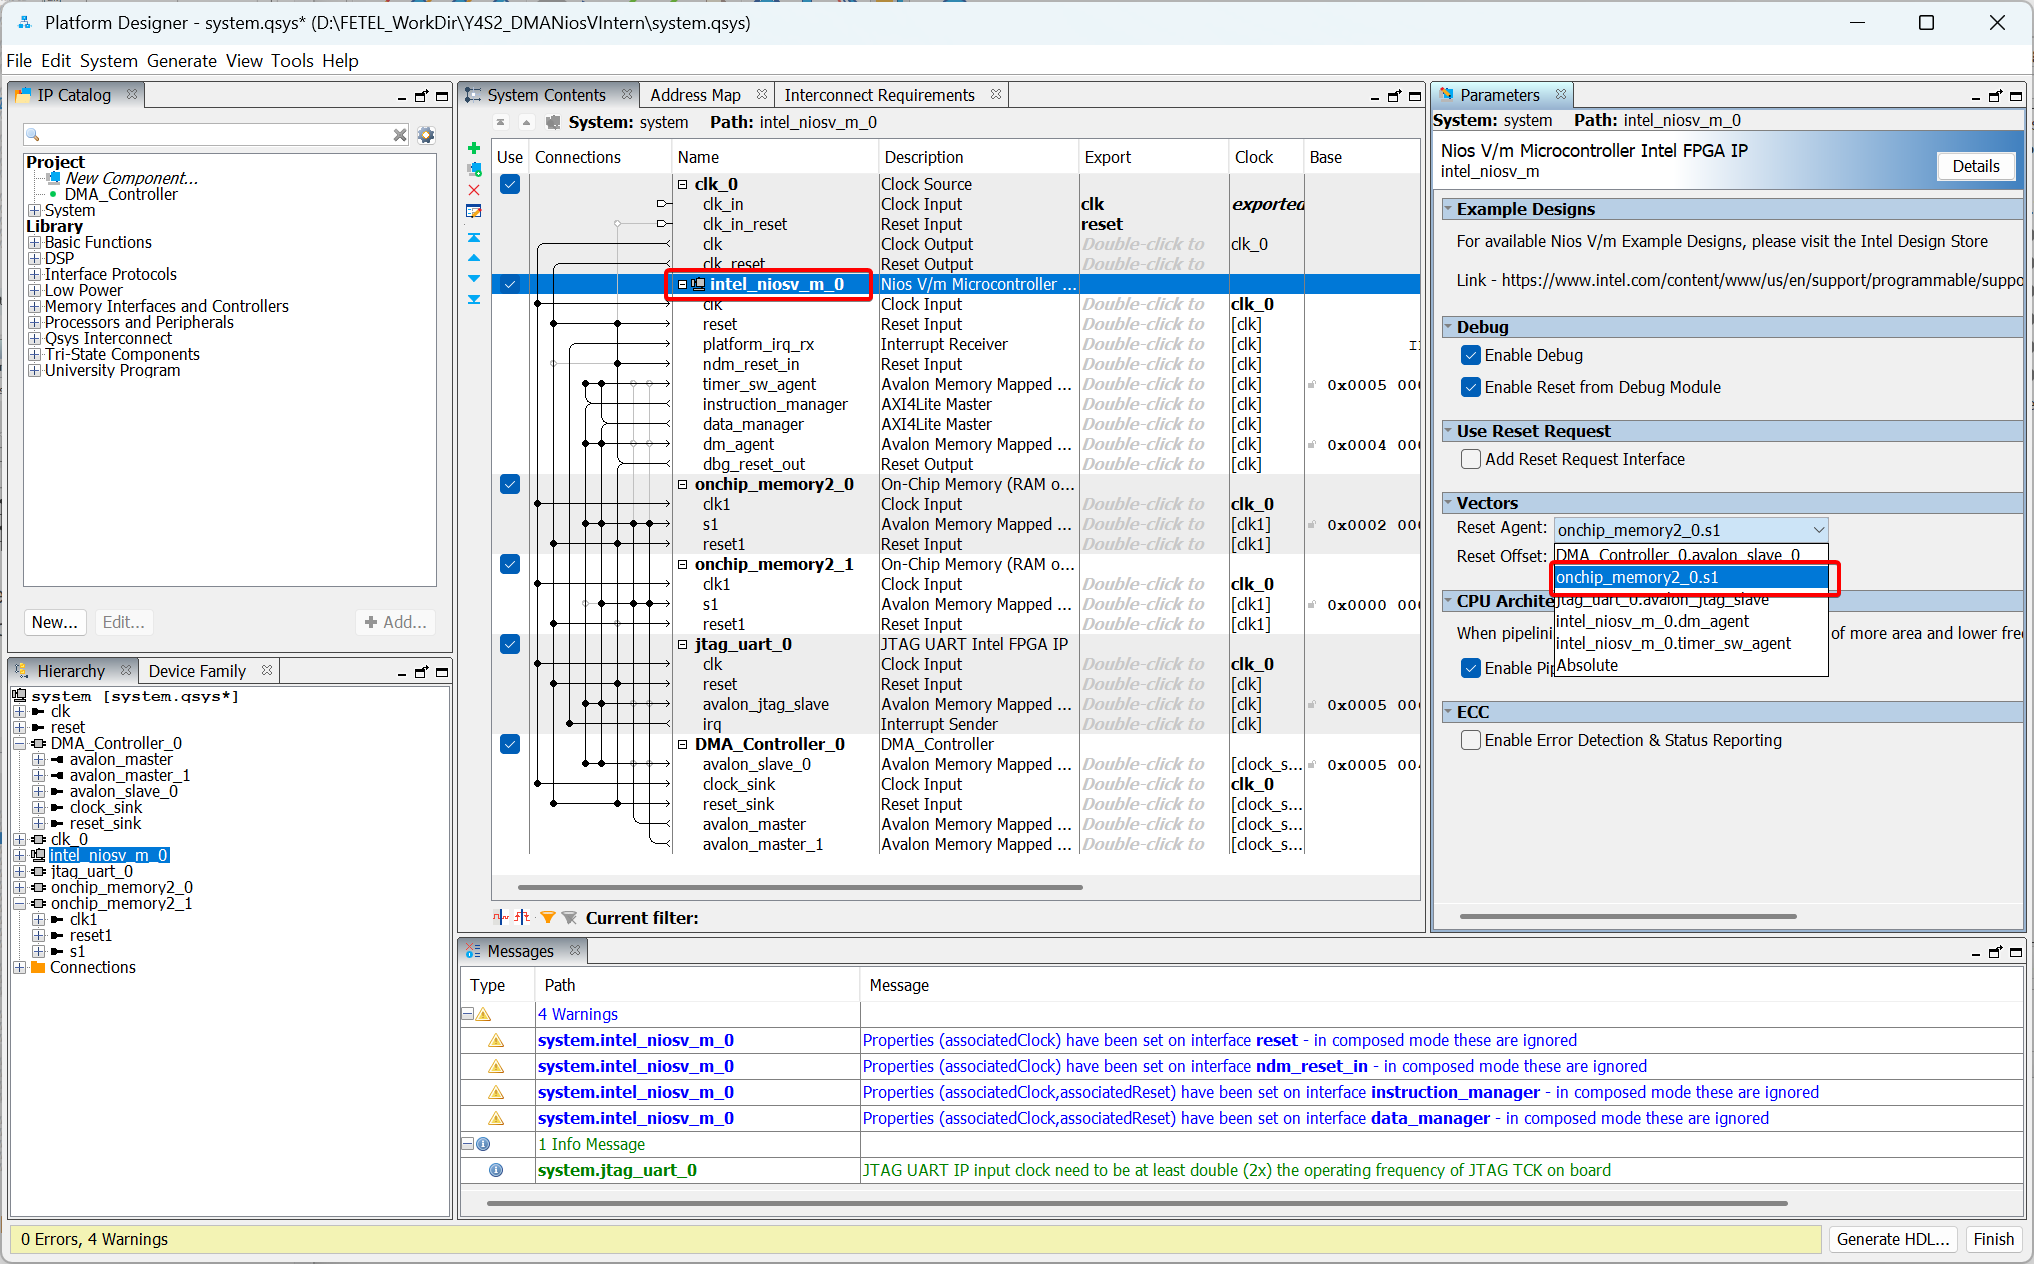
\includegraphics[width=\linewidth]
{03_31_NiosVVectorConfig.png} \caption{Cấu hình IP Nios V/m: Đặt Bộ nhớ Vector Reset (Reset Vector Memory).} \label{fig:03_31} \end{figure}
% \begin{figure}[htbp] \centering 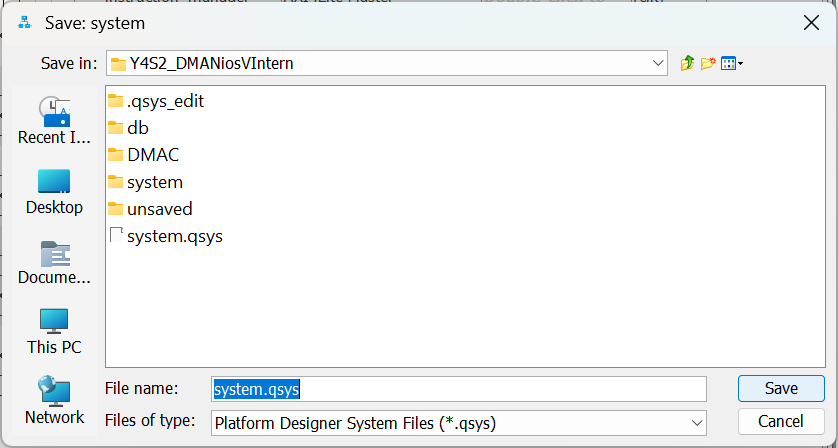
\includegraphics[width=0.5\linewidth]{03_32_PlatformDesignerSaveSystem.png} \caption{Platform Designer: Lưu hệ thống thành system.qsys.} \label{fig:03_32} \end{figure}
% \begin{figure}[htbp] \centering 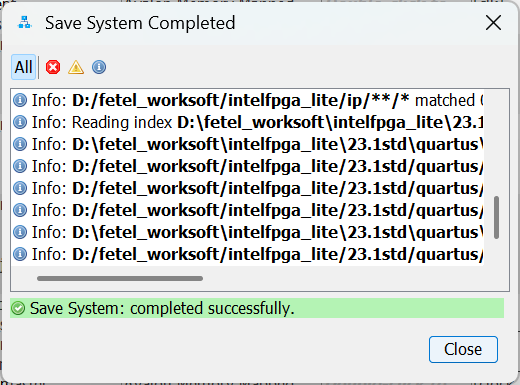
\includegraphics[width=0.5\linewidth]{03_33_PlatformDesignerSaveComplete.png} \caption{Platform Designer: Thông báo lưu hệ thống thành công.} \label{fig:03_33} \end{figure}
\begin{figure}[htbp] \centering 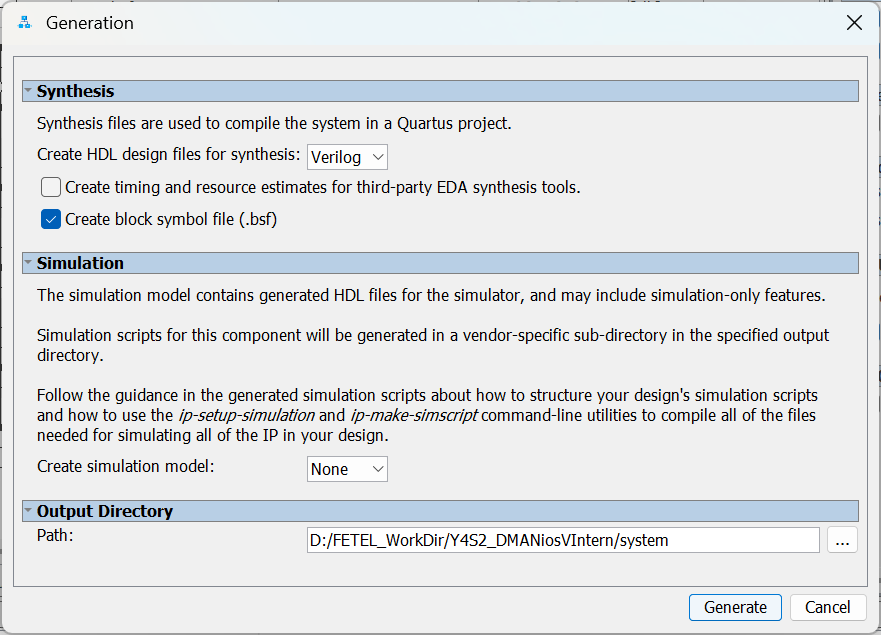
\includegraphics[width=0.7\linewidth]{03_34_PlatformDesignerGenerateHDL.png} \caption{Platform Designer: Hộp thoại Tạo HDL (Generate HDL).} \label{fig:03_34} \end{figure}
% \begin{figure}[htbp] \centering 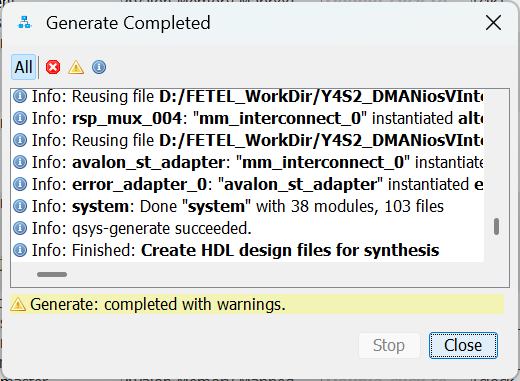
\includegraphics[width=0.4\linewidth]{03_35_PlatformDesignerGenerateComplete.png} \caption{Platform Designer: Thông báo hoàn thành tạo HDL.} \label{fig:03_35} \end{figure}
% \begin{figure}[htbp] \centering 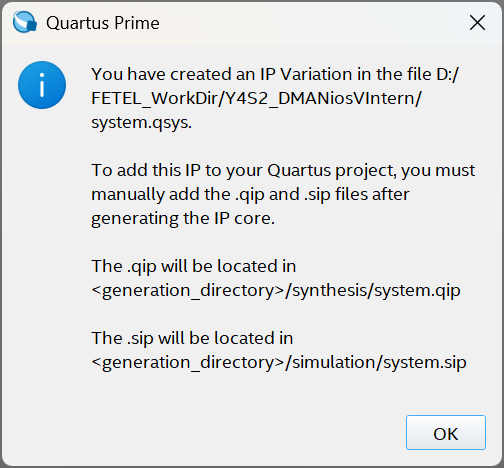
\includegraphics[width=0.4\linewidth]{03_36_QuartusAddGeneratedIPInfo.png} \caption{Quartus: Thông báo đề xuất thêm tệp .qip đã tạo.} \label{fig:03_36} \end{figure}
\begin{figure}[htbp] \centering 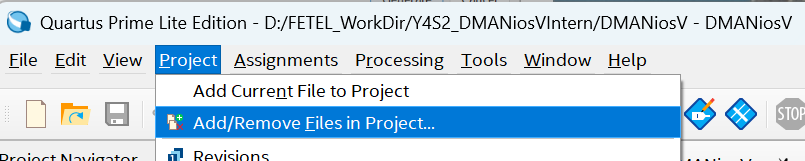
\includegraphics[width=0.8\linewidth]{03_37_QuartusAddFilesToProjectMenu.png} \caption{Quartus: Menu Project -> Add/Remove Files in Project...} \label{fig:03_37} \end{figure}
\begin{figure}[htbp] \centering 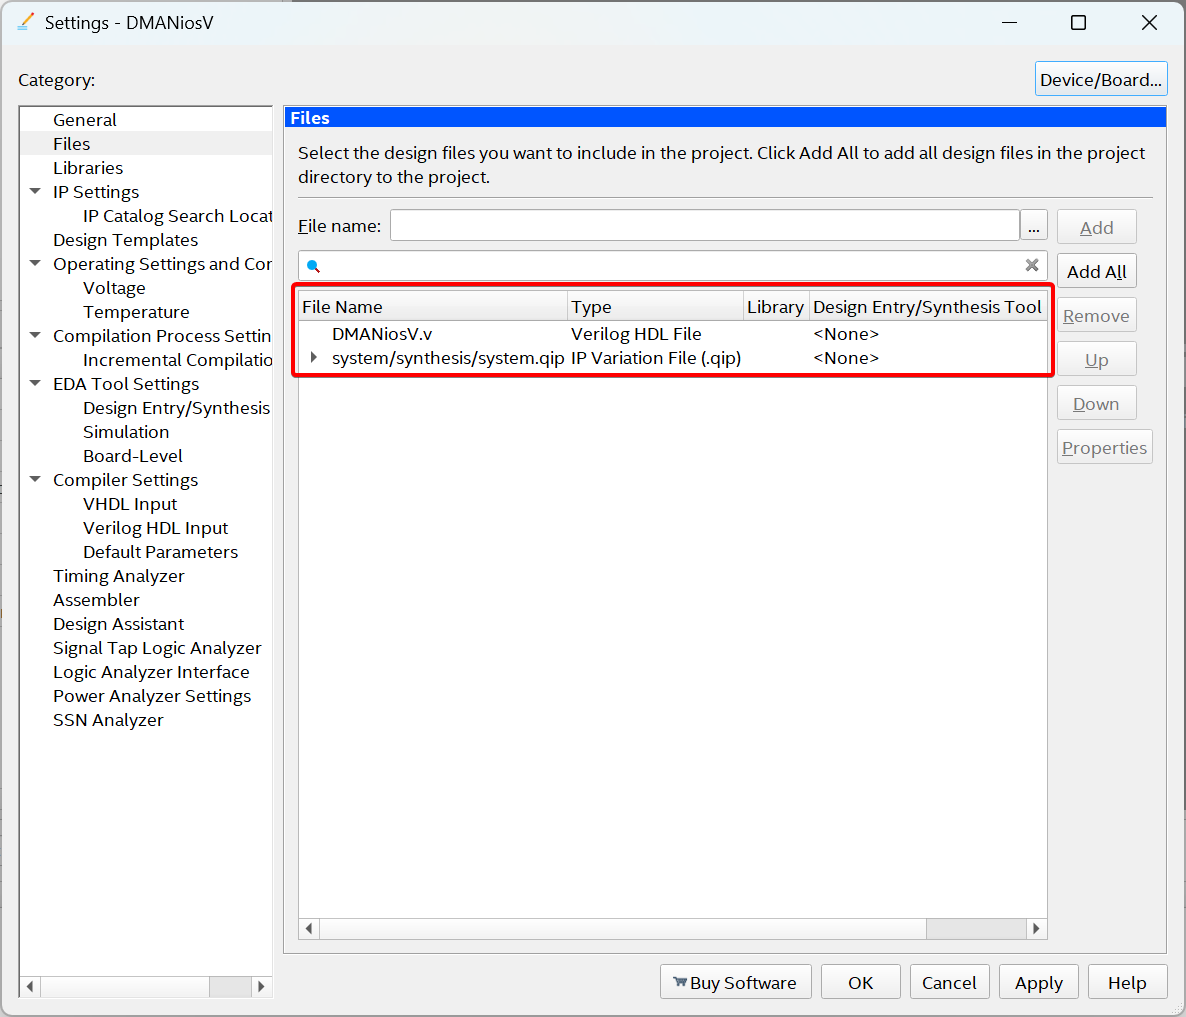
\includegraphics[width=0.7\linewidth]{03_38_QuartusProjectFilesSettings.png} \caption{Quartus: Cài đặt Dự án - Cửa sổ Tệp hiển thị tệp .qip đã thêm.} \label{fig:03_38} \end{figure}
\begin{figure}[htbp] \centering 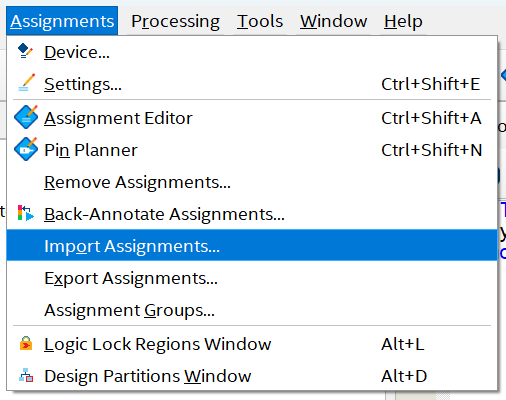
\includegraphics[width=0.5\linewidth]{03_39_QuartusImportAssignmentsMenu.png} \caption{Quartus: Menu Assignments -> Import Assignments...} \label{fig:03_39} \end{figure}
\begin{figure}[htbp] \centering 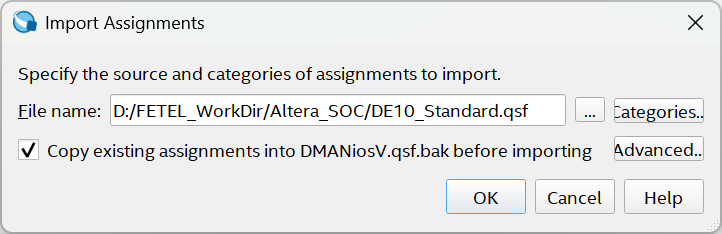
\includegraphics[width=0.5\linewidth]{03_40_QuartusImportAssignmentsDialog.png} \caption{Quartus: Hộp thoại Nhập Gán chân (Import Assignments) để chọn tệp .qsf.} \label{fig:03_40} \end{figure}
\begin{figure}[htbp] \centering 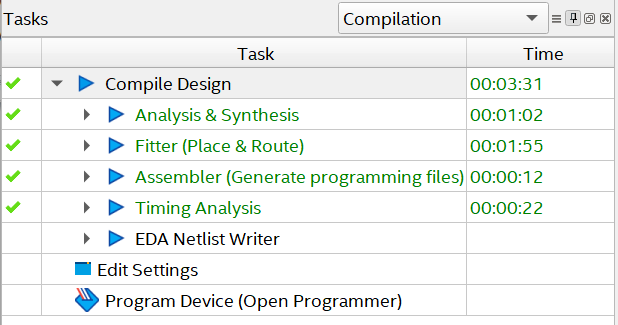
\includegraphics[width=0.6\linewidth]{03_41_QuartusCompilationTasks.png} \caption{Quartus: Compile Design thành công.} \label{fig:03_41} \end{figure}
\begin{figure}[htbp] \centering 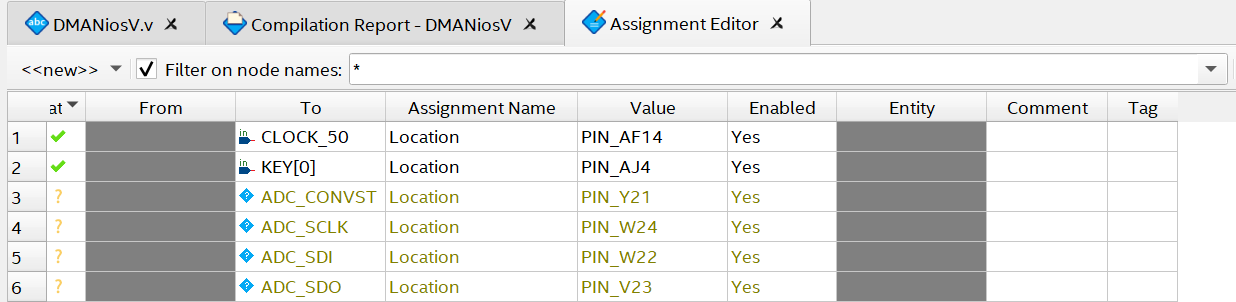
\includegraphics[width=\linewidth]{03_42_QuartusAssignmentEditor.png} \caption{Quartus: Trình chỉnh sửa Gán chân (Assignment Editor) hiển thị các gán chân đã nhập.} \label{fig:03_42} \end{figure}

\FloatBarrier

\section{Phát triển Ứng dụng Phần mềm Nios V}
\label{sec:develop_software}

Phần này mô tả việc tạo Gói Hỗ trợ Bo mạch (Board Support Package - \acrshort{bsp}) và mã ứng dụng C, sau đó biên dịch và gỡ lỗi (debug) nó bằng \acrshort{ide} Ashling RiscFree.

\begin{enumerate}
    \item \textbf{Chuẩn bị Cấu trúc Thư mục Phần mềm:} Tạo một thư mục \texttt{software} trong thư mục dự án chính (\texttt{DMANiosVIntern}). Bên trong \texttt{software}, tạo hai thư mục con: \texttt{app} và \texttt{bsp} (Hình \ref{fig:03_43}). Đặt mã nguồn ứng dụng C của bạn (ví dụ: \texttt{source.c} chứa logic kiểm thử DMA) vào bên trong thư mục \texttt{app} (Hình \ref{fig:03_45}).
    \item \textbf{Tạo BSP và Tệp CMake:}
    \begin{itemize}
        \item Mở Nios V command shell (\texttt{niosv-shell.exe}) nằm trong thư mục cài đặt Intel FPGA (ví dụ: \texttt{intelFPGA\_lite/23.1std/niosv/bin}) (Hình \ref{fig:03_46}).
        \item Điều hướng Nios V Shell đến thư mục dự án (Working Directory, \ref{fig:03_11}): 
        \begin{lstlisting}[language=bash, caption={Điều hướng trong Nios V Shell}, label=lst:cd_project] 
        cd D:\FETEL_WorkDir\Y4S2_DMANiosVIntern \end{lstlisting}
        \item Tạo \acrshort{bsp} bằng lệnh \texttt{niosv-bsp}. Lệnh này sử dụng tệp thông tin phần cứng (\texttt{.sopcinfo}) được tạo bởi Platform Designer để tạo các trình điều khiển (drivers) và các tệp tiêu đề hệ thống (system headers) \cite{intelNiosVSoftwareDevHandbook}:
        \begin{lstlisting}[language=bash, caption={Lệnh tạo BSP Nios V}, label=lst:gen_bsp]
# -c: create BSP, -t=hal: type HAL, --sopcinfo: path to hardware info
niosv-bsp -c -t=hal --sopcinfo=system.sopcinfo software/bsp/settings.bsp \end{lstlisting}
        \item Tạo các tệp xây dựng CMake cho ứng dụng bằng \texttt{niosv-app}. Lệnh này liên kết nguồn ứng dụng (\texttt{-a}) với \acrshort{bsp} đã tạo (\texttt{-b}) và chỉ định thư mục nguồn (\texttt{-s}) \cite{intelNiosVSoftwareDevHandbook}:
        \begin{lstlisting}[language=bash, caption={Lệnh tạo tệp CMake ứng dụng Nios V}, label=lst:gen_app]
# -a: app dir, -b: bsp dir, -s: source dir (relative to app dir)
niosv-app -a=software/app -b=software/bsp -s=software/app \end{lstlisting}
        (Xem Hình \ref{fig:03_47} cho việc thực thi lệnh và Hình \ref{fig:03_48} cho đầu ra tạo BSP). Đảm bảo không có lỗi xảy ra. Một tệp \texttt{CMakeLists.txt} bây giờ sẽ tồn tại trong thư mục \texttt{software/app}.
    \end{itemize}
    \item \textbf{Xây dựng Ứng dụng bằng Ashling RiscFree™ IDE \cite{ashling_riscfree_guide}:}
    \begin{itemize}
        \item \textbf{Khởi chạy IDE:} Quan trọng là khởi chạy Ashling RiscFree™ IDE từ \texttt{ niosv-shell.exe} bằng cách gõ \texttt{riscfree}. Điều này đảm bảo các biến môi trường (environment variables) được thiết lập chính xác (Hình \ref{fig:03_49}).
        \item \textbf{Chọn Workspace:} Chọn thư mục \texttt{software} (Hình \ref{fig:03_50}).
        \item \textbf{Import Project:} Trong IDE (Hình \ref{fig:03_51}), đi đến File -> New -> C/C++ Project (Hình \ref{fig:03_52}). Chọn "C Project". Đặt tên dự án là \texttt{app} (trùng với tên thư mục). Chọn "Empty Project" dưới loại dự án "CMake driven" (Hình \ref{fig:03_53}). Nhấp Finish. IDE sẽ phát hiện \texttt{CMakeLists.txt} và cấu hình dự án.
        \item \textbf{Xây dựng Dự án (Build Project):} Nhấp chuột phải vào dự án \texttt{app} trong Trình khám phá Dự án (Project Explorer) (Hình \ref{fig:03_54}) và chọn "Build Project" (hoặc sử dụng Ctrl+B) (Hình \ref{fig:03_55}). Kiểm tra cửa sổ Console để xem tiến trình xây dựng và đảm bảo nó hoàn thành mà không có lỗi (Hình \ref{fig:03_56}). Thao tác này tạo ra tệp thực thi (\texttt{app.elf}) bên trong một thư mục xây dựng (ví dụ: \texttt{software/app/build/Debug}). 
    \end{itemize}
    \item \textbf{Nạp chương trình cho FPGA và Chạy/Gỡ lỗi Phần mềm:}
    \begin{itemize}
        \item \textbf{Nạp chương trình cho FPGA (Program FPGA):} Sử dụng Quartus Programmer (Tools -> Programmer) để tải thiết kế phần cứng đã biên dịch (tệp \texttt{.sof} từ mục \ref{sec:build_hardware}) lên bo mạch DE10-Standard thông qua kết nối \acrshort{usb}-Blaster. Đảm bảo phần cứng đã được kết nối và bắt đầu quá trình nạp (Hình \ref{fig:03_59}).
        \item \textbf{Cấu hình Trình gỡ lỗi (Configure Debugger):} Trong Ashling IDE, nhấp chuột phải vào dự án \texttt{app} -> Run As -> Ashling RISC-V Hardware Debugging... (Hình \ref{fig:03_60}). Chọn app.elf (Hình \ref{fig:03_61}).
        \begin{itemize}
            \item Chuyển đến tab "Debugger". Chọn Đầu dò Gỡ lỗi (Debug Probe) chính xác (ví dụ: "DE-SoC [\acrshort{usb}-1]"). Đảm bảo "Lựa chọn Thiết bị/TAP (Device/TAP selection)" khớp với lõi Nios V được xác định trên chuỗi \acrshort{jtag} (sử dụng "Auto-detect Scan Chain" nếu không chắc chắn). Loại Vận chuyển (Transport type) phải là \acrshort{jtag} (Hình \ref{fig:03_62}). Áp dụng (Apply) và nhấp Debug.
        \end{itemize}
        \item \textbf{Chạy và Quan sát (Run and Observe):} IDE sẽ kết nối với lõi Nios V, tải xuống tệp \texttt{.elf}, và dừng tại đầu hàm \texttt{main()} (Hình \ref{fig:03_63}). Mở một \texttt{juart-terminal} trong Nios V shell để xem đầu ra (output) của chương trình:
        \begin{lstlisting}[language=bash, caption={Khởi chạy JTAG UART Terminal}, label=lst:juart]
juart-terminal \end{lstlisting}
        \item Quan sát đầu ra trong cửa sổ \texttt{juart-terminal} (Hình \ref{fig:03_64}, \ref{fig:03_65}, \ref{fig:03_66}). Đầu ra ví dụ cho thấy các thanh ghi DMA đang được cấu hình, trạng thái đang được thăm dò (polling), bộ đệm bộ nhớ đang được xóa/xả (cleared/flushed), và cuối cùng, xác minh rằng việc truyền dữ liệu qua DMA đã diễn ra chính xác.
    \end{itemize}
\end{enumerate}

% Figure environments for Section 3.3
\begin{figure}[htbp] \centering 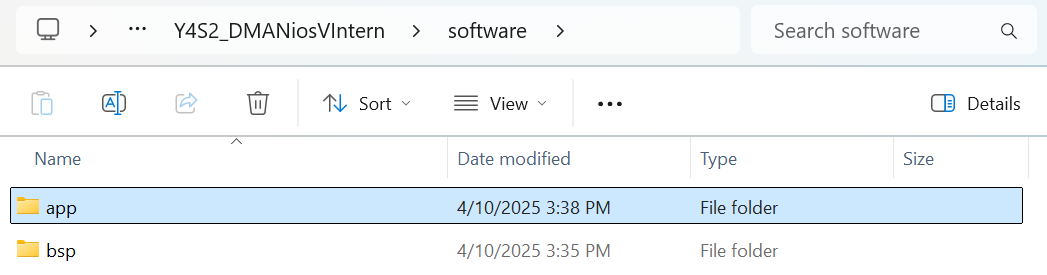
\includegraphics[width=0.8\linewidth]{03_43_SoftwareFoldersAppBSP.png} \caption{Cấu trúc thư mục Software gồm các thư mục con \texttt{app} và \texttt{bsp}.} \label{fig:03_43} \end{figure}
\begin{figure}[htbp] \centering 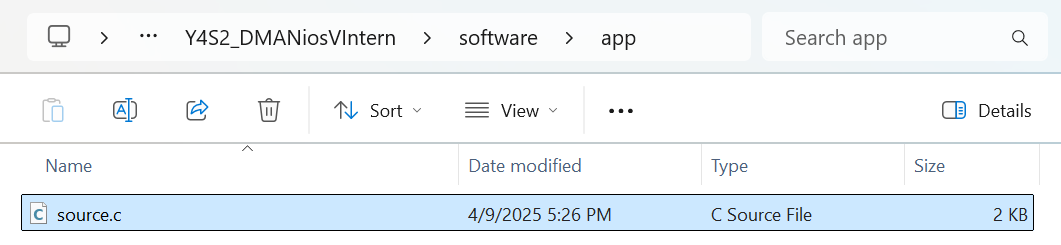
\includegraphics[width=0.8\linewidth]{03_45_SoftwareAppFolderSourceC.png} \caption{Thư mục \texttt{software/app} chứa tệp mã nguồn \texttt{source.c}.} \label{fig:03_45} \end{figure}
\begin{figure}[htbp] \centering 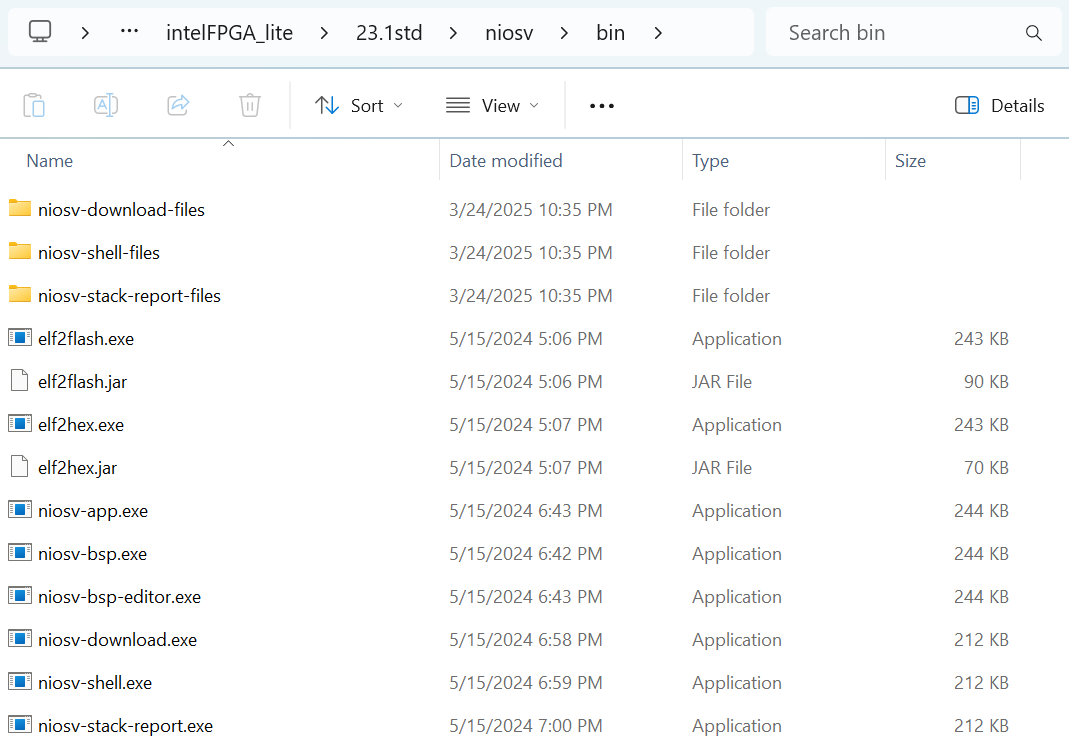
\includegraphics[width=0.8\linewidth]{03_46_NiosVShellLocation.png} \caption{Vị trí của \texttt{niosv-shell.exe}.} \label{fig:03_46} \end{figure}
\begin{figure}[htbp] \centering 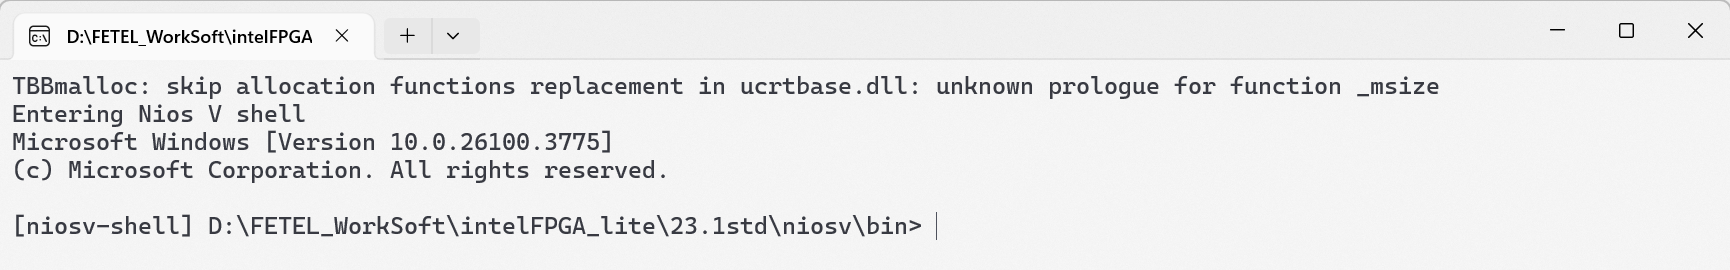
\includegraphics[width=\linewidth]{03_47_NiosVShellCommands.png} \caption{Cửa sổ Nios V Shell.} \label{fig:03_47} \end{figure}
\begin{figure}[htbp] \centering 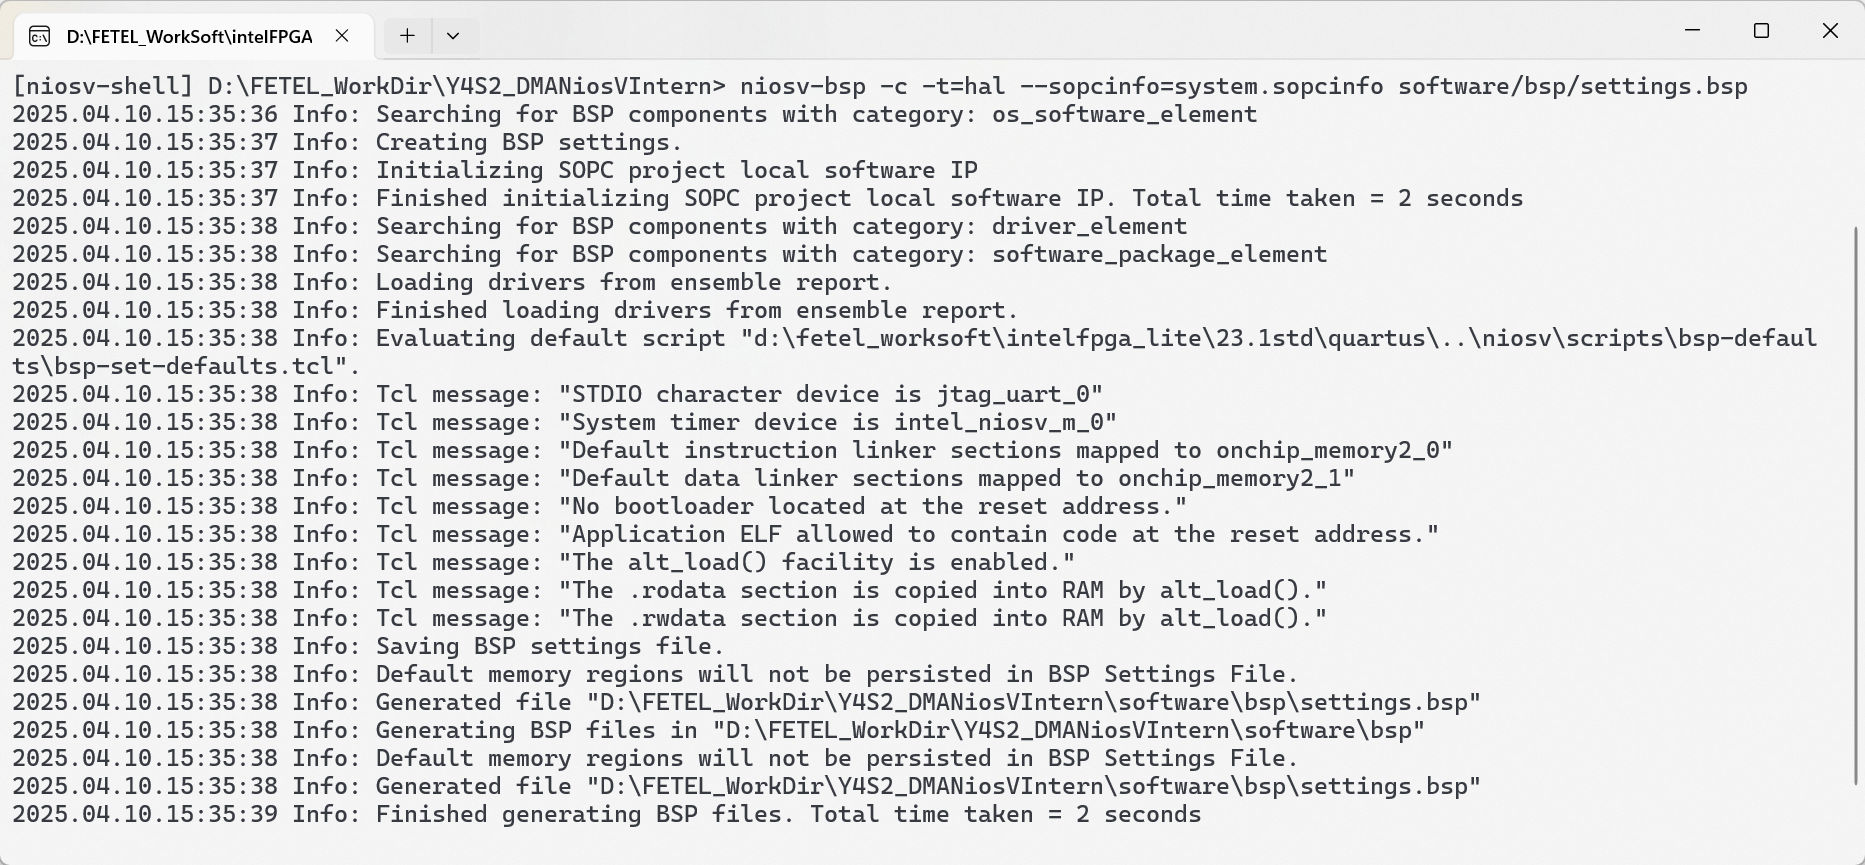
\includegraphics[width=\linewidth]{03_48_NiosVShellBSPOutput.png} \caption{Đầu ra từ việc thực thi lệnh \texttt{niosv-bsp}.} \label{fig:03_48} \end{figure}\begin{figure}[htbp] \centering 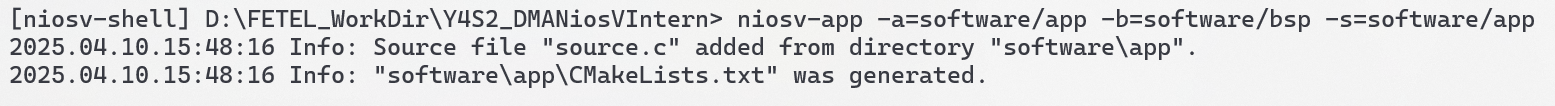
\includegraphics[width=0.9\linewidth]{03_49_NiosVShellAppOutput.png} \caption{Đầu ra từ việc thực thi lệnh \texttt{niosv-app}.} \label{fig:03_49} \end{figure}
\begin{figure}[htbp] \centering 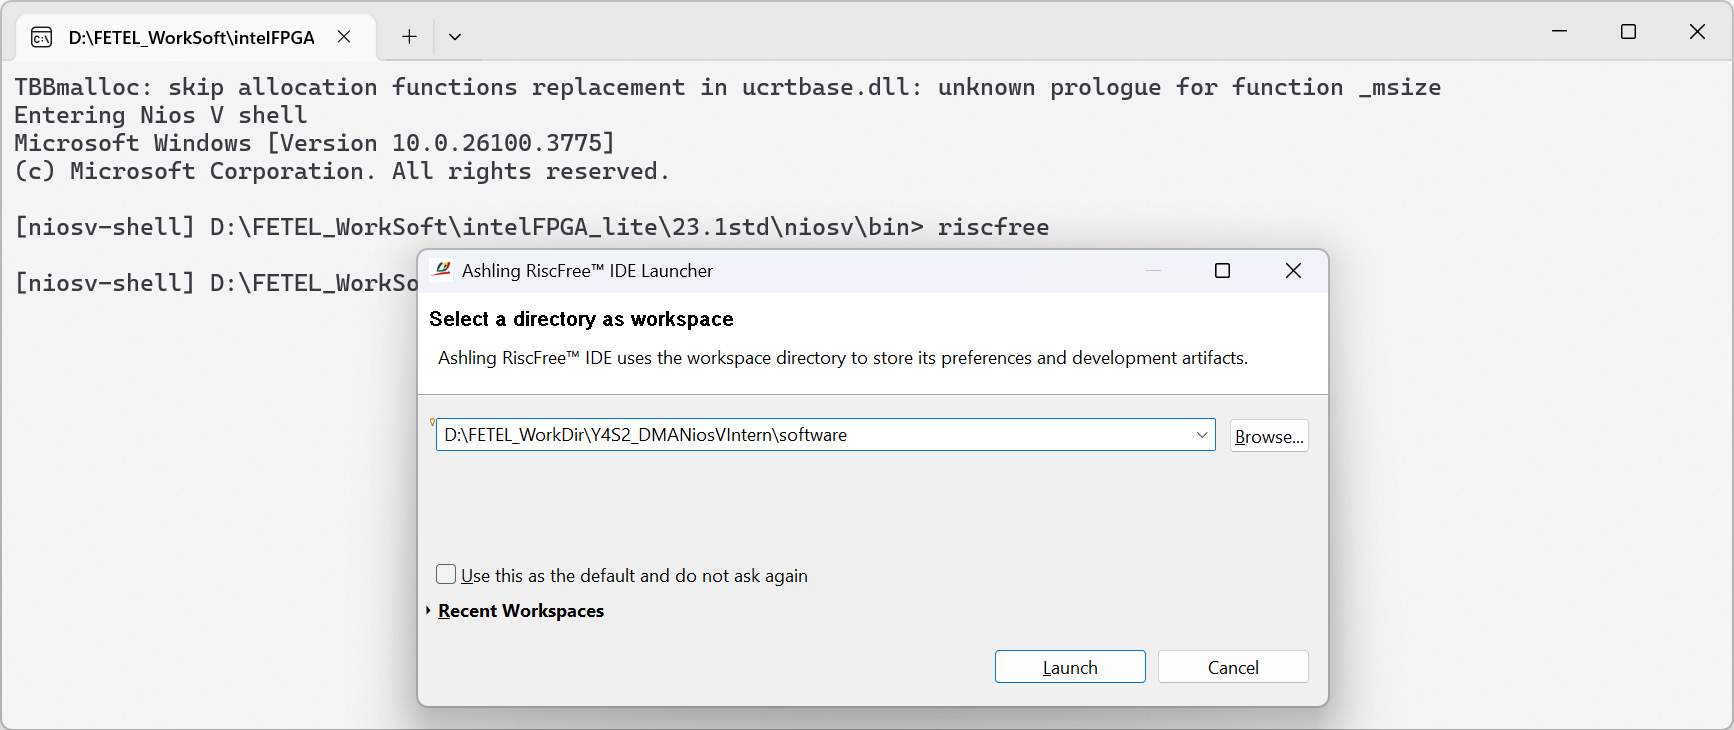
\includegraphics[width=\linewidth]{03_50_AshlingRiscFreefromNiosVShell.png} \caption{Khởi chạy Ashling RiscFree™ IDE từ Nios V Shell, chọn đường dẫn Workspace.} \label{fig:03_50} \end{figure}
\begin{figure}[htbp] \centering 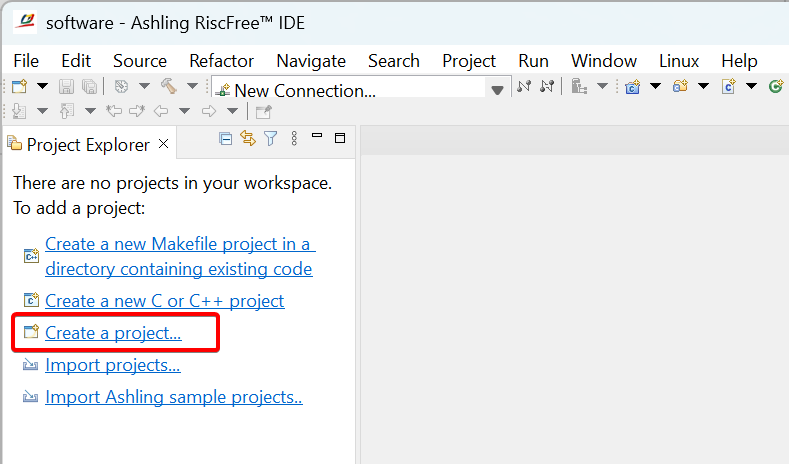
\includegraphics[width=0.8\linewidth]{03_51_AshlingRiscFreeLauncher2.png} \caption{Màn hình chào mừng Ashling RiscFree™ IDE: Chọn "Create a project...".} \label{fig:03_51} \end{figure}
\begin{figure}[htbp] \centering 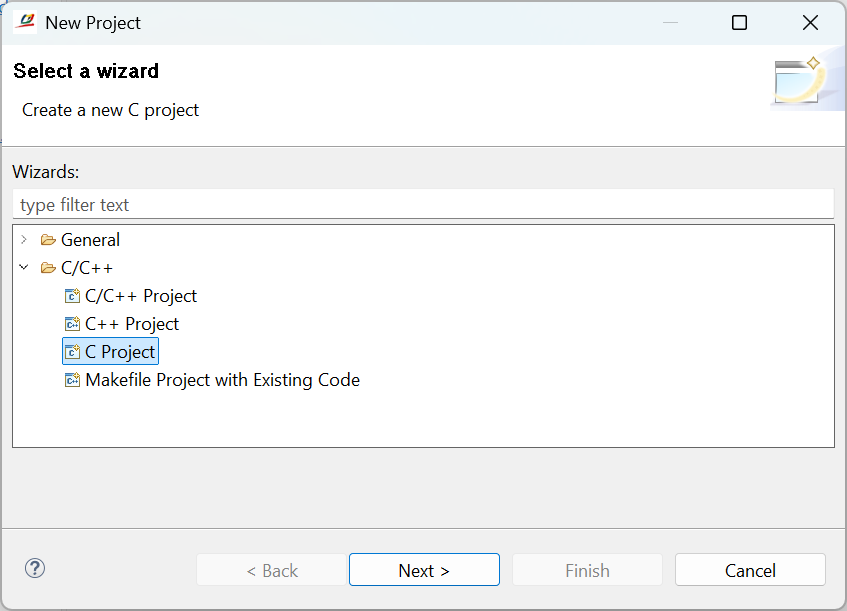
\includegraphics[width=0.8\linewidth]{03_52_AshlingIDEWelcome.png} \caption{Ashling IDE: Chọn C/C++ $\longrightarrow$ C Project.} \label{fig:03_52} \end{figure}
\begin{figure}[htbp] \centering 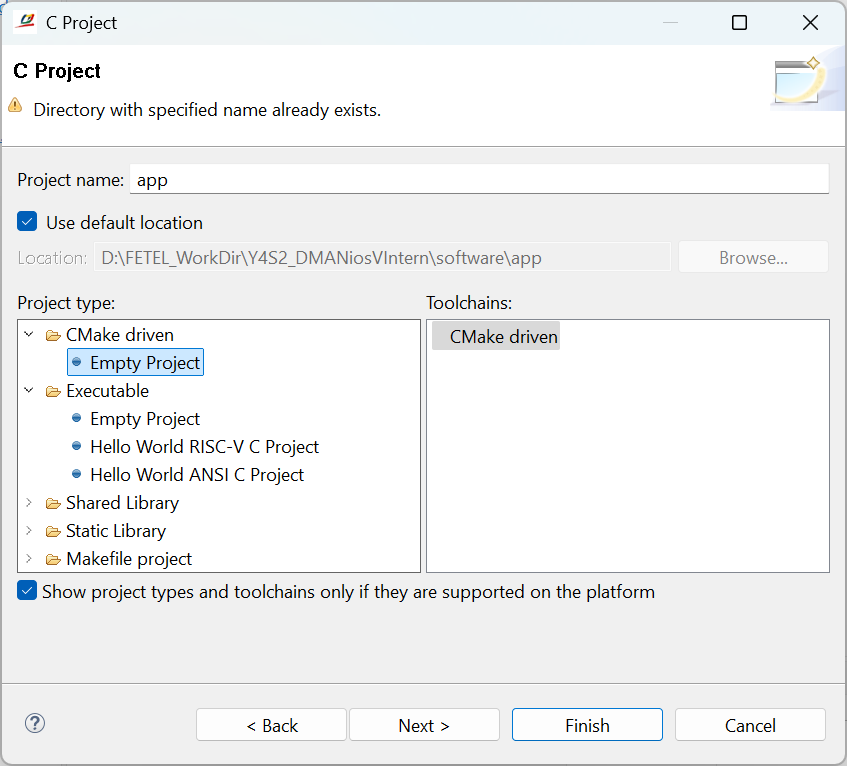
\includegraphics[width=0.8\linewidth]{03_53_AshlingIDENewProjectWizard1.png} \caption{Ashling IDE: Chọn CMake driven $\longrightarrow$ Empty Project.} \label{fig:03_53} \end{figure}
\begin{figure}[htbp] \centering 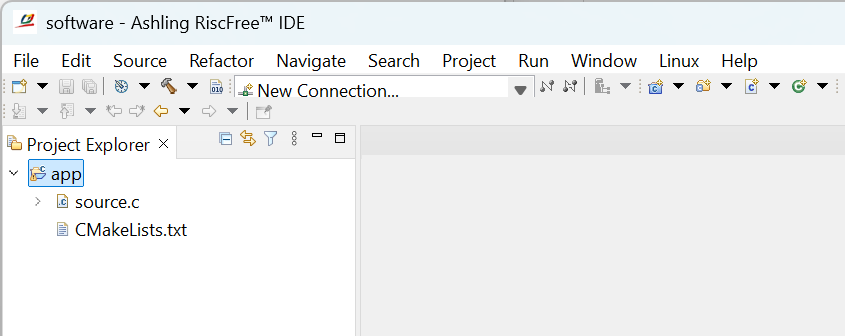
\includegraphics[width=0.8\linewidth]{03_54_AshlingIDENewProjectWizard2.png} \caption{Ashling IDE: Project Explorer hiển thị dự án 'app'.} \label{fig:03_54} \end{figure}
\begin{figure}[htbp] \centering 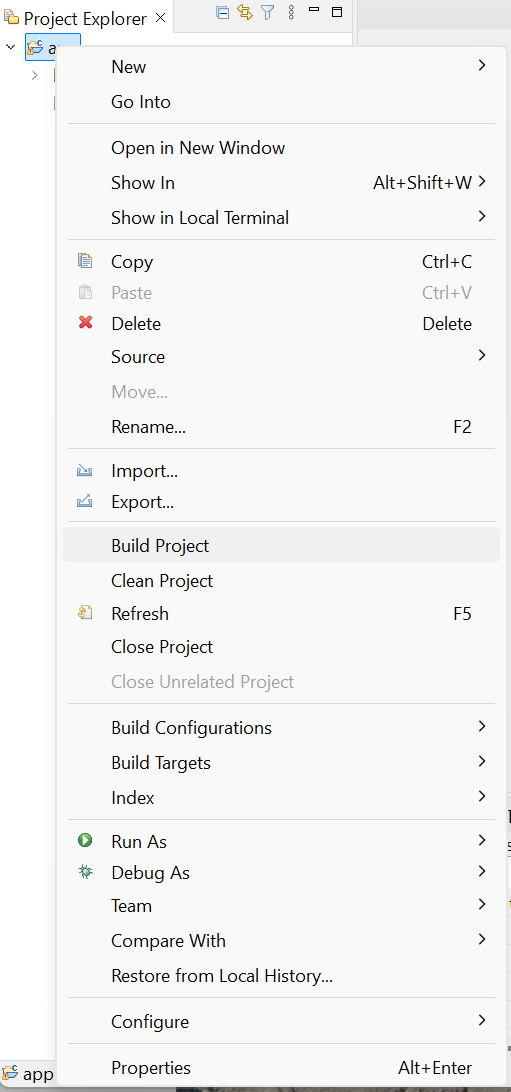
\includegraphics[width=0.4\linewidth]{03_55_AshlingIDEProjectExplorer.png} \caption{Ashling IDE: nhấp chuột phải 'app' $\longrightarrow$ Build Project.} \label{fig:03_55} \end{figure}
\begin{figure}[htbp] \centering 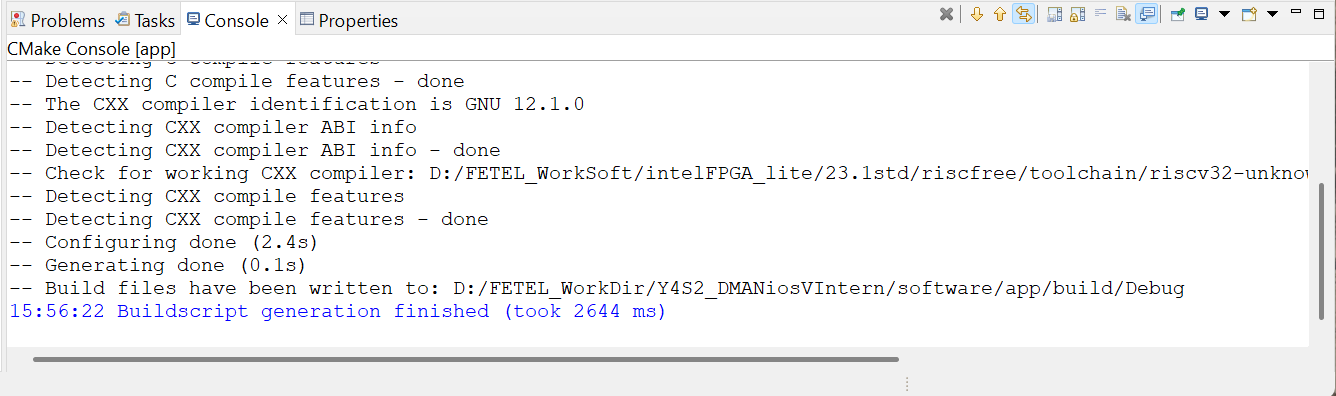
\includegraphics[width=\linewidth]{03_56_AshlingIDEBuildMenu.png} \caption{Ashling IDE: Console thông báo Build thành công.} \label{fig:03_56} \end{figure}
% \begin{figure}[htbp] \centering 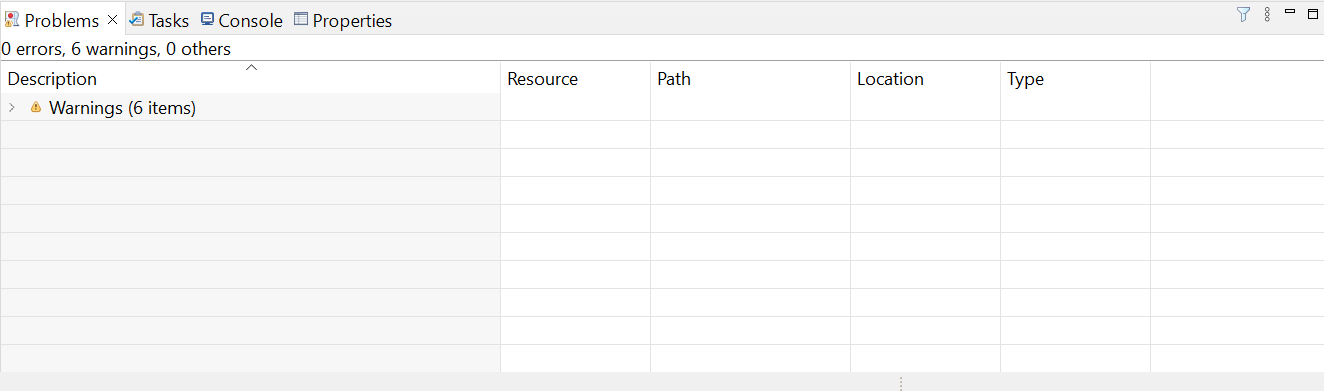
\includegraphics[width=0.8\linewidth]{03_57_AshlingIDEBuildConsole.png} \caption{Ashling IDE: Tab Problems không có lỗi.} \label{fig:03_57} \end{figure}
% \begin{figure}[htbp] \centering 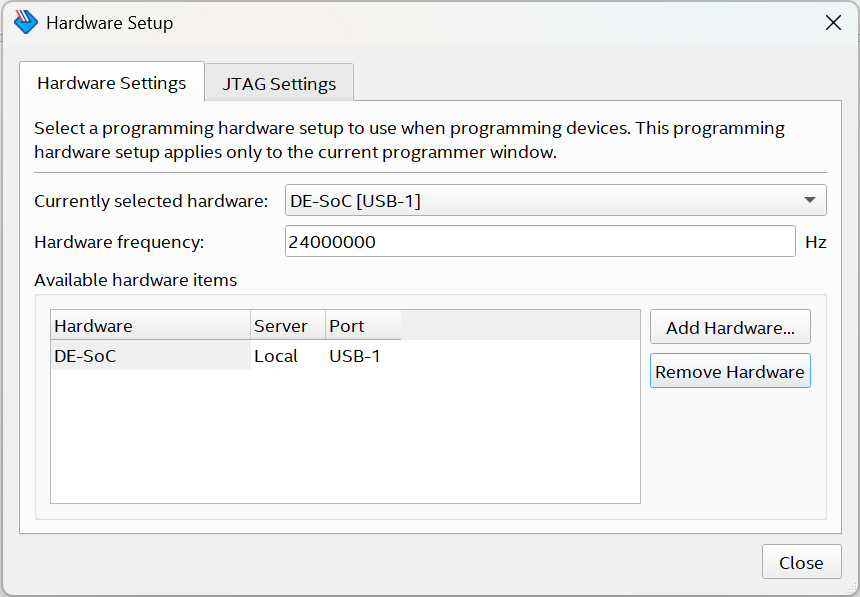
\includegraphics[width=0.6\linewidth]{03_58_QuartusProgrammerSetup.png} \caption{Trình lập trình Quartus: Cửa sổ Cài đặt Phần cứng (Hardware Setup) hiển thị DE-SoC đã được nhận.} \label{fig:03_58} \end{figure}
\begin{figure}[htbp] \centering 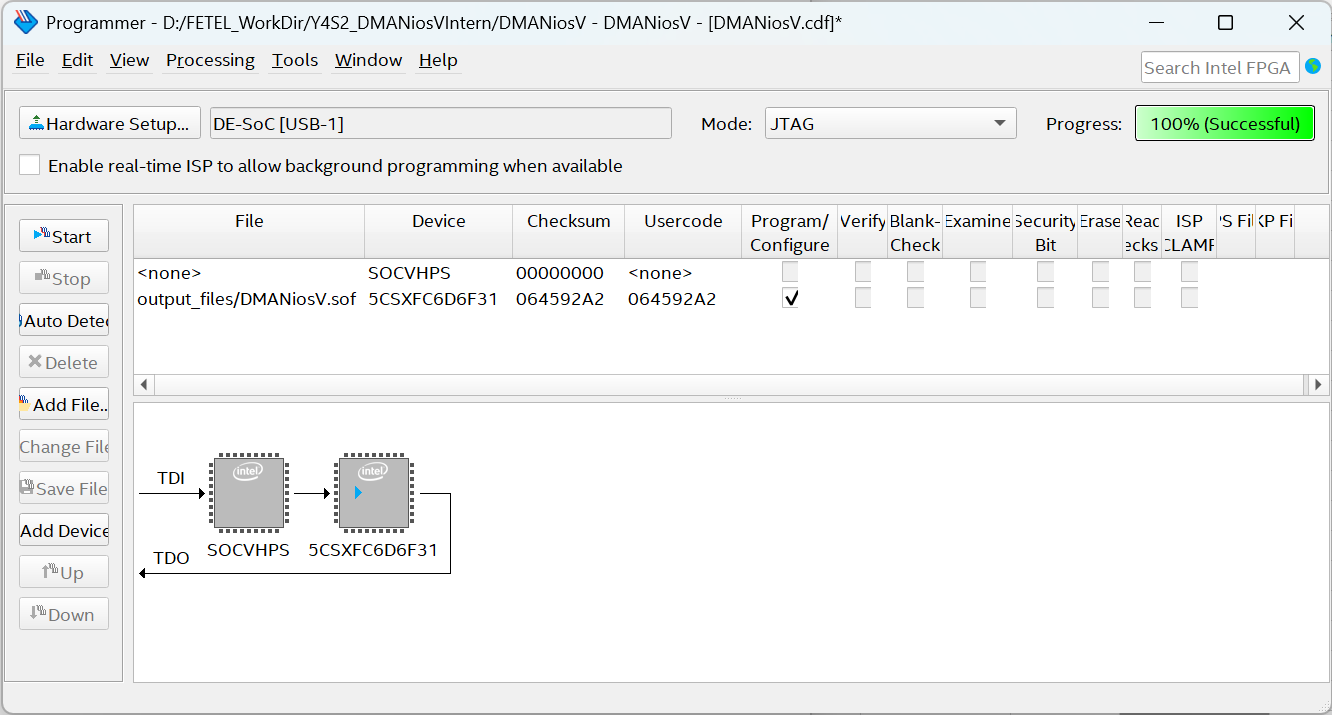
\includegraphics[width=0.7\linewidth]{03_59_QuartusProgrammerWindow.png} \caption{Quartus Programmer: Nạp tệp .sof xuống board thành công.} \label{fig:03_59} \end{figure}
\begin{figure}[htbp] \centering 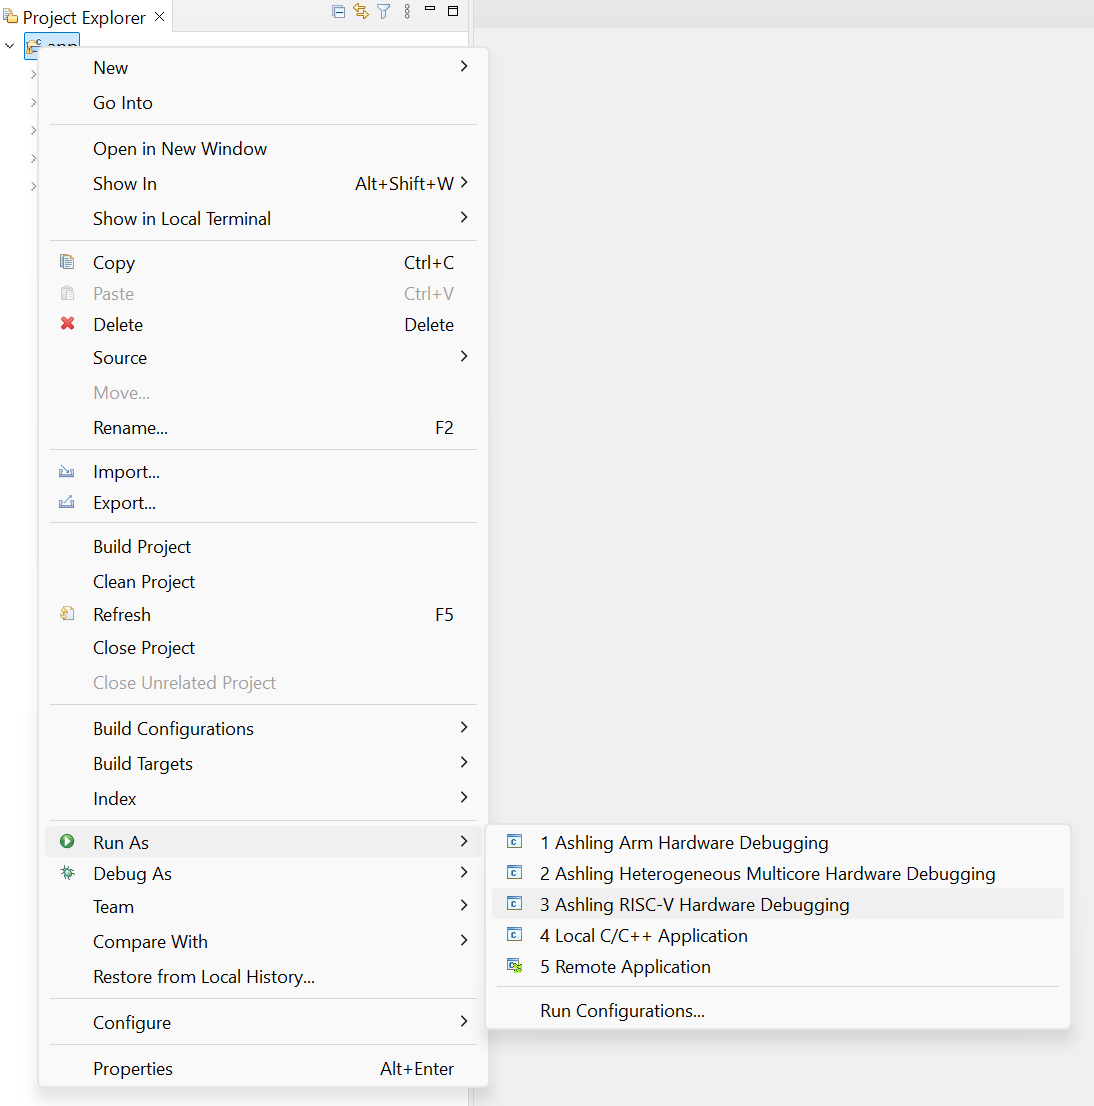
\includegraphics[width=0.8\linewidth]{03_60_AshlingIDEDebugMenu.png} \caption{Ashling IDE: Nạp Firmware xuống lõi Nios V (Run As $\longrightarrow$ Ashling RISC-V Hardware Debugging.} \label{fig:03_60} \end{figure}
\begin{figure}[htbp] \centering 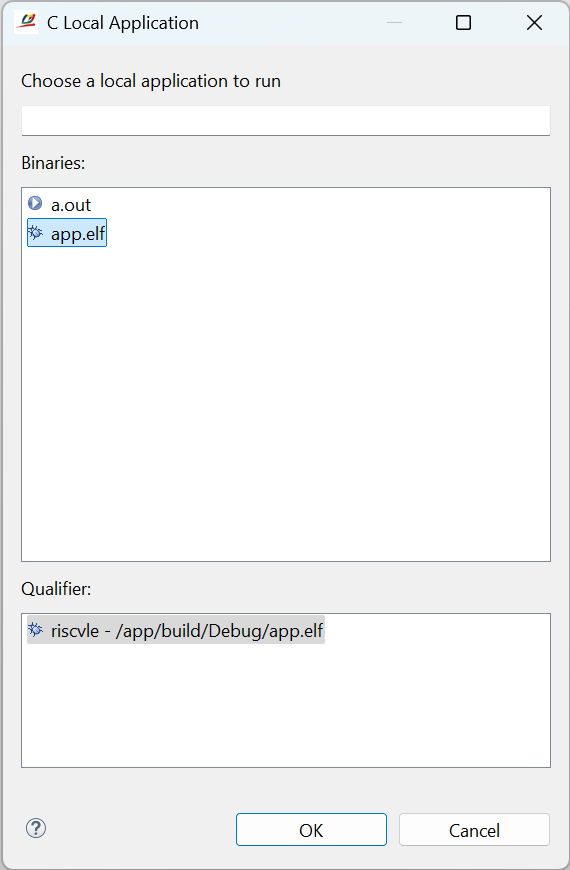
\includegraphics[width=0.4\linewidth]{03_61_AshlingIDERunConfigELF.png} \caption{Ashling IDE: Cấu hình Gỡ lỗi - Chỉ định ứng dụng C/C++ (.elf).} \label{fig:03_61} \end{figure}
\begin{figure}[htbp] \centering \includegraphics[width=\linewidth]{03_62_AshlingIDEDebugConfig.png} \caption{Ashling IDE: Cấu hình Gỡ lỗi - Cài đặt tab Debugger.} \label{fig:03_62} \end{figure}
\begin{figure}[htbp] \centering \includegraphics[width=\linewidth]{03_63_AshlingIDEDebugConsole.png} \caption{Ashling IDE: Debug Console cho biết đang chờ kết nối (Nhấn nút đỏ để ngừng chạy).} \label{fig:03_63} \end{figure}
\begin{figure}[htbp] \centering \includegraphics[width=0.8\linewidth]{03_64_JUARTTerminalOutput1.png} \caption{Đầu ra JTAG UART Terminal: Thông báo ban đầu và reset DMA.} \label{fig:03_64} \end{figure}
\begin{figure}[htbp] \centering \includegraphics[width=0.8\linewidth]{03_65_JUARTTerminalOutput2.png} \caption{Đầu ra JTAG UART Terminal: Trạng thái bộ đệm và cấu hình DMA.} \label{fig:03_65} \end{figure}
\begin{figure}[htbp] \centering \includegraphics[width=0.7\linewidth]{03_66_JUARTTerminalOutput3.png} \caption{Đầu ra JTAG UART Terminal: Xác minh truyền DMA thành công.} \label{fig:03_66} \end{figure}

\FloatBarrier

% Platform Designer có thể tạo ra các mô hình mô phỏng (simulation models) (Hình \ref{fig:03_34}), nhưng việc tạo ra một hệ thống bàn thử nghiệm (testbench system) đầy đủ, đặc biệt là liên quan đến các mô hình bộ xử lý như Nios V/g, có thể phức tạp và đôi khi gặp hạn chế về công cụ trên hệ điều hành Windows cho việc tạo testbench \cite{intel-forum-simulation}.

% Note: Appendix content moved to appendix1.tex as per user's template structure
% References moved to references.bib